\documentclass[11pt]{article}

\usepackage[a4paper,margin=2.25cm]{geometry}
\usepackage{amsmath,amssymb,bm}
\usepackage{booktabs,longtable,array,tabularx}
\usepackage{graphicx}
\usepackage{xcolor}
\usepackage{microtype}
\usepackage[hidelinks]{hyperref}
\usepackage[nameinlink,noabbrev]{cleveref}

\graphicspath{{../reference_results/figures/}}
\crefname{figure}{Supplementary Figure}{Supplementary Figures}
\Crefname{figure}{Supplementary Figure}{Supplementary Figures}

\newcommand{\angstrom}{\text{\AA}}
\newcommand{\dd}{\mathrm{d}}
\newcommand{\COM}{\mathrm{COM}}
\newcommand{\PBC}{\mathrm{PBC}}
\newcommand{\NPBC}{\mathrm{NPBC}}
\newcommand{\OO}{\mathrm{OO}}
\newcommand{\OH}{\mathrm{OH}}
\newcommand{\HH}{\mathrm{HH}}
\newcommand{\mean}[1]{\left\langle #1\right\rangle}

\title{Supplementary Information\\[0.5em]
Detailed computation of the structural, thermodynamic, radial-distribution,
and interfacial observables for frozen-bias spherical water cavities}
\author{Giuseppe Stefano Basile}
\date{22 September 2026}

\begin{document}
\maketitle

\begin{abstract}
This document gives the complete analysis protocol used to compare water in
spherical non-periodic cavities of radius 15, 20, and \(30\,\angstrom\)
(R15, R20, and R30) with a matched periodic reference.  It defines the
trajectory windows, molecular reconstruction, radial shell estimators,
orientational and network observables, temporal fluctuation convention,
frozen Gaussian mean-field reconstruction, boundary-safe and radially
resolved radial distribution functions (RDFs), molecule- and volume-weighted
histograms, practical-equivalence screen, experimental RDF comparison, and
all numerical quality-control checks.  The aim is to make every quantity in
\crefrange{fig:s01-density}{fig:s28-js} reproducible from the archived trajectories and
tables without relying on plotting-code defaults.
\end{abstract}

\tableofcontents

\section{Systems, trajectories, and analysis windows}

\subsection{Frozen-bias NPBC cavities and periodic reference}

The three non-periodic systems contain only water and are confined within
spherical cavities.  The molecular mean-field biases were frozen before the
validation trajectories used here.  The final frozen profiles correspond to
global optimizer updates 159 (R15), 212 (R20), and 188 (R30).  The nominal
target number density was
\begin{equation}
  \rho_0 = 0.037242\ \text{molecules}\,\angstrom^{-3}.
\end{equation}
The actual geometric densities calculated from \(N/(4\pi R^3/3)\) are given
in \cref{tab:systems}.  The periodic reference, denoted PBC40, contains 2383
water molecules in a cubic cell of side \(40.000\,\angstrom\), and therefore
has number density \(0.037234375\,\angstrom^{-3}\).  It used the same
MACE--OFF23 \texttt{small\_2} potential as the reference production run.

\begin{table}[htbp]
\centering
\caption{Systems used in the validation analysis.  The outer-volume
fractions are exact geometric fractions of a sphere.}
\label{tab:systems}
\begin{tabular}{lrrrrr}
\toprule
System & \(R\) (\(\angstrom\)) & Waters & \(\rho\) (\(\angstrom^{-3}\))
& outer 2 \(\angstrom\) & outer 5 \(\angstrom\) \\
\midrule
R15 & 15 & 526  & 0.037207 & 0.349037 & 0.703704 \\
R20 & 20 & 1248 & 0.037242 & 0.271000 & 0.578125 \\
R30 & 30 & 4211 & 0.037233 & 0.186963 & 0.421296 \\
PBC40 & --- & 2383 & 0.037234375 & --- & --- \\
\bottomrule
\end{tabular}
\end{table}

For a spherical cavity, the fraction of volume within a distance \(a\) of
the wall is
\begin{equation}
 f_{\mathrm{outer}}(a;R)
 = 1-\left(1-\frac{a}{R}\right)^3,
 \qquad 0\leq a\leq R.
 \label{eq:outer-volume}
\end{equation}
Equation~\eqref{eq:outer-volume} was used in the surface-to-volume comparison
shown in \cref{fig:s16-equivalence-geometry}.

\subsection{Trajectory assembly}

LAMMPS custom dumps were parsed frame by frame.  The required columns were
the molecule identifier, atom type, and Cartesian coordinates
\texttt{mol type x y z}.  Atom type 1 was oxygen and atom type 2 was
hydrogen.  Each molecule was required to contain exactly one oxygen and two
hydrogens.  Frames failing this topology check, the expected molecule count,
or the expected sampling grid were rejected.

R30 was stored in two trajectory files.  A step offset of 550000 was applied
to the second segment before sorting and duplicate removal.  Thus the two
segments were treated as one ordered validation record without altering their
coordinates.  All molecular and pair observables were recomputed directly
from the atomic coordinates; no trajectory-averaged observable was read from
a LAMMPS log.

\subsection{Two sampling conventions}

Two deliberately distinct sampling conventions were retained because they
serve different purposes.

\paragraph{Whole-radius validation (\crefrange{fig:s01-density}{fig:s16-equivalence-geometry}).}
The complete endpoints were included.  Each NPBC system contributed 201
frames separated by 5 ps over a nominal 1 ns interval:
R15 and R30 used 100--1100 ps, whereas R20 used 0--1000 ps.  Per-frame
temporal standard deviations in these figures were therefore calculated from
all 201 frames.  Regional block estimates used ten nominal 100 ps blocks; the
inclusive final endpoint was assigned to the tenth block.

\paragraph{Matched RDF extension (\crefrange{fig:s17-goo-exp}{fig:s21-goo-full-exp}).}
RDFs were sampled every 25 ps.  R15, R20, and R30 each contributed 41 frames,
including both endpoints.  PBC40 contributed 33 frames over 200--1000 ps.
The first temporal standard deviation was calculated from nominal 100 ps RDF
blocks.

\paragraph{Final radial-layer analysis (\crefrange{fig:s22-radial-goo}{fig:s28-js}).}
To make every temporal block exactly equal, half-open windows were used:
\begin{align}
 \mathrm{R15}:&\ [100,1100)\ \mathrm{ps}, & n_f&=200,\\
 \mathrm{R20}:&\ [0,1000)\ \mathrm{ps},   & n_f&=200,\\
 \mathrm{R30}:&\ [100,1100)\ \mathrm{ps},& n_f&=200,\\
 \mathrm{PBC40}:&\ [200,1000)\ \mathrm{ps},& n_f&=160.
\end{align}
Frames were separated by 5 ps.  Each 100 ps block consequently contained 20
frames, giving ten blocks for each NPBC system and eight blocks for PBC40.
This half-open convention is the definitive convention for the radial-layer
RDFs, shell histograms, and their temporal fluctuation bands.

\section{Molecular reconstruction and single-molecule observables}

\subsection{Molecular center of mass and radial coordinate}

With \(m_{\mathrm O}=15.999\) and \(m_{\mathrm H}=1.008\), the center of mass
of water molecule \(i\) was
\begin{equation}
 \bm R_i^{\COM} =
 \frac{m_{\mathrm O}\bm R_{i\mathrm O}
 +m_{\mathrm H}(\bm R_{i\mathrm H_1}+\bm R_{i\mathrm H_2})}
 {m_{\mathrm O}+2m_{\mathrm H}}.
 \label{eq:com}
\end{equation}
Its absolute radial coordinate and distance from the wall were
\begin{equation}
 r_i=\left|\bm R_i^{\COM}\right|,
 \qquad d_i=R-r_i.
 \label{eq:wall-distance}
\end{equation}
For radial-layer assignment only, negative values caused by very small
one-step overshoots were clipped to zero.  Overshoot counts and maximum
overshoots were retained as quality-control observables.

\subsection{Dipole, bond, and molecular-plane orientation}

The unnormalized molecular dipole-bisector direction was
\begin{equation}
 \bm b_i=\frac{\bm R_{i\mathrm H_1}+\bm R_{i\mathrm H_2}}{2}
 -\bm R_{i\mathrm O},
\end{equation}
and the outward radial unit vector was
\(\hat{\bm r}_i=\bm R_i^{\COM}/r_i\).  The primary orientational variable was
\begin{equation}
 \cos\theta_i=\hat{\bm b}_i\cdot\hat{\bm r}_i.
\end{equation}
Legendre order parameters were evaluated molecule by molecule as
\begin{equation}
 P_{\ell,i}=P_\ell(\cos\theta_i),\qquad \ell=1,\ldots,6.
 \label{eq:legendre}
\end{equation}
The water-plane normal was
\begin{equation}
 \hat{\bm n}_i=
 \frac{(\bm R_{i\mathrm H_1}-\bm R_{i\mathrm O})\times
       (\bm R_{i\mathrm H_2}-\bm R_{i\mathrm O})}
 {|(\bm R_{i\mathrm H_1}-\bm R_{i\mathrm O})\times
       (\bm R_{i\mathrm H_2}-\bm R_{i\mathrm O})|},
\end{equation}
and its second-rank radial order was
\(P_2(\hat{\bm n}_i\cdot\hat{\bm r}_i)\).  Finally, the bond order parameters
were the average over the two unit O--H bonds,
\begin{equation}
 P_\ell^{\mathrm{bond}}(i)=\frac12\sum_{a=1}^{2}
 P_\ell(\hat{\bm e}_{ia}\cdot\hat{\bm r}_i),\qquad \ell=1,2.
 \label{eq:bond-order}
\end{equation}
Undefined directions at the exact cavity center were stored as missing values
and excluded only from the affected orientational average.
The full-radius dipole profiles are reported in \cref{fig:s02-orientation},
and their volume-weighted distributions are included in
\cref{fig:s13-distributions}.

\subsection{Intramolecular geometry}

The two O--H lengths were \(l_{ia}=|\bm R_{i\mathrm H_a}-\bm R_{i\mathrm O}|\).
The reported mean bond length and H--O--H angle were
\begin{align}
 \overline l_{\OH,i}&=\frac12(l_{i1}+l_{i2}),\\
 \alpha_i&=\cos^{-1}(\hat{\bm e}_{i1}\cdot\hat{\bm e}_{i2}).
 \label{eq:intra}
\end{align}
Angles were converted to degrees.
The radial means and shell-conditioned distributions are shown in
\cref{fig:s04-intramolecular,fig:s26-intra-hists}, respectively.

\subsection{Nearest-neighbor distances and coordination}

A Cartesian \texttt{cKDTree} of oxygen positions was constructed for each
NPBC frame.  For every water, the first through fifth distinct oxygen-neighbor
distances were retained as \(d_{1,\OO},\ldots,d_{5,\OO}\).  The coordination
number was the direct count
\begin{equation}
 N_{\OO,i}(3.5)=\sum_{j\ne i}
 \Theta(3.5\,\angstrom-r_{ij}^{\OO}).
 \label{eq:coord}
\end{equation}
For PBC40, the same calculation used a periodic \texttt{cKDTree} with a
\(40\,\angstrom\) box and minimum-image distances.
The radial first- and fourth-neighbor means are shown in
\cref{fig:s05-neighbors}; the complete first-through-fifth distributions are
shown in \cref{fig:s27-neighbor-hists}.

\subsection{Tetrahedral order}

Let \(\hat{\bm u}_{ij}\) denote the unit vector from oxygen \(i\) to one of
its four nearest oxygen neighbors.  The tetrahedral order parameter was
\begin{equation}
 q_i=1-\frac{3}{8}\sum_{j=1}^{3}\sum_{k=j+1}^{4}
 \left(\hat{\bm u}_{ij}\cdot\hat{\bm u}_{ik}+\frac13\right)^2.
 \label{eq:tetra}
\end{equation}
The periodic calculation applied the minimum-image convention to all four
neighbor vectors before evaluating \cref{eq:tetra}.
Tetrahedrality enters the radial network profiles in \cref{fig:s03-network}
and the layer-resolved distributions in \cref{fig:s25-network-hists}.

\subsection{Hydrogen bonds}

A directional hydrogen bond \(i\rightarrow j\) was assigned when
\begin{equation}
 r_{ij}^{\OO}\leq3.5\,\angstrom
 \quad\text{and}\quad
 \angle(\mathrm O_i-\mathrm H_{ia}\cdots\mathrm O_j)\geq150^\circ
 \label{eq:hbond}
\end{equation}
for either hydrogen \(a\) of donor \(i\).  Donated and accepted bonds were
counted separately, and their sum was reported as the total hydrogen-bond
count per molecule.  Periodic O--O and O--H vectors were minimum-imaged before
the angular test.
The resulting hydrogen-bond profiles and distributions are displayed in
\cref{fig:s03-network,fig:s25-network-hists}.

\section{Radial profiles, density, and temporal fluctuations}

\subsection{Spherical shells}

The complete cavity was partitioned into shells of width
\(\Delta r=0.25\,\angstrom\).  Shell \(s\), bounded by \(r_s^-\) and
\(r_s^+\), had exact volume
\begin{equation}
 V_s=\frac{4\pi}{3}\left[(r_s^+)^3-(r_s^-)^3\right].
 \label{eq:shell-volume}
\end{equation}
Molecules were assigned by their COM radius.  If \(n_s(t)\) is the number of
molecular centers in shell \(s\) at saved frame \(t\), the normalized density
was
\begin{equation}
 \widetilde\rho_s(t)=\frac{n_s(t)}{V_s\rho_0}.
 \label{eq:density}
\end{equation}
The displayed profile is the arithmetic temporal mean of
\(\widetilde\rho_s(t)\).  For a generic per-molecule property \(A_i(t)\), the
per-frame shell mean was
\begin{equation}
 A_s(t)=\frac{\sum_i A_i(t)\,\mathbf 1[i\in s]}
 {\sum_i\mathbf 1[i\in s]}.
 \label{eq:frame-shell-mean}
\end{equation}
Empty shell frames were stored as missing values rather than as zero.
The density and other full-radius shell means obtained from these estimators
are plotted in \crefrange{fig:s01-density}{fig:s05-neighbors}.

\subsection{First temporal standard deviation}

For a shell with \(n_s^{\mathrm{valid}}\) finite frame values, the first
temporal standard deviation was
\begin{equation}
 \sigma_{t,s}(A)=
 \sqrt{\frac{1}{n_s^{\mathrm{valid}}-1}
 \sum_{t}\left[A_s(t)-\overline A_s\right]^2}.
 \label{eq:temporal-sd}
\end{equation}
Every shaded band labelled ``\(\pm1\sigma_t\)'' is
\(\overline A_s\pm\sigma_{t,s}(A)\).  It is not a standard error or a
confidence interval.  The corresponding temporal SEM stored in the tables is
\(\sigma_{t,s}/\sqrt{n_s^{\mathrm{valid}}}\).  The valid-frame fraction was
also recorded; shells occupied in fewer than 50\% of frames were explicitly
marked in the full-radius plots.

The shell count variance and Fano factor were
\begin{equation}
 F_s=\frac{\operatorname{Var}_t[n_s(t)]}{\mean{n_s(t)}_t},
 \label{eq:fano}
\end{equation}
using the sample variance with one degree of freedom.
The radial fluctuation profiles are collected in
\cref{fig:s10-density-potential,fig:s12-temporal-sd}; all shaded bands in
\crefrange{fig:s01-density}{fig:s05-neighbors} use the same convention.

\section{Global translational and angular-isotropy diagnostics}

The displacement of the instantaneous water COM cloud from the cavity origin
was quantified by
\begin{equation}
 \Delta_{\COM}(t)=
 \left|\frac{1}{N}\sum_{i=1}^{N}\bm R_i^{\COM}(t)\right|.
 \label{eq:global-com}
\end{equation}
Angular isotropy was measured from
\begin{equation}
 \bm M(t)=\frac1N\sum_i\hat{\bm r}_i\hat{\bm r}_i^{\mathsf T},
 \qquad
 \bm Q(t)=\frac32\bm M(t)-\frac12\bm I.
 \label{eq:q-tensor}
\end{equation}
The reported diagnostics were the Frobenius norm
\(\|\bm Q\|_F=[\operatorname{Tr}(\bm Q^{\mathsf T}\bm Q)]^{1/2}\) and the
three ordered eigenvalues of \(\bm Q\).  A perfectly isotropic distribution
has \(\bm Q=\bm 0\).  Frame means, frame SDs, 100 ps block means, block SEMs,
and block-bootstrap pairwise differences were retained.
The corresponding global time traces and summary bands are shown in
\cref{fig:s11-global}.

\section{Molecule-weighted and shell-volume-weighted distributions}

Four radial regions were defined by the shell-midpoint wall distance
\(d_s=R-r_s^{\mathrm{mid}}\): the complete cavity; interior
\(d_s\geq5\,\angstrom\); outer 5 \(\angstrom\), \(d_s<5\,\angstrom\); and
outer 2 \(\angstrom\), \(d_s<2\,\angstrom\).

Let \(h_{sj}\) be the count in histogram bin \(j\) for shell \(s\).  The
molecule-weighted probability was
\begin{equation}
 p_j^{\mathrm{mol}}=
 \frac{\sum_{s\in\mathcal R}h_{sj}}
 {\sum_{s\in\mathcal R}\sum_k h_{sk}}.
 \label{eq:molecule-weighted}
\end{equation}
For volume weighting, each occupied shell histogram was first normalized,
\(p_{sj}=h_{sj}/\sum_kh_{sk}\), and then averaged with exact shell-volume
weights,
\begin{equation}
 p_j^{\mathrm{vol}}=
 \sum_{s\in\mathcal R}w_s p_{sj},
 \qquad
 w_s=\frac{V_s}{\sum_{u\in\mathcal R}^{\mathrm{occupied}}V_u}.
 \label{eq:volume-weighted}
\end{equation}
Thus molecule weighting answers ``what distribution is observed for a random
molecule?'', whereas volume weighting gives equal physical-volume importance
to the spherical shells and prevents the larger population of outer shells
from dominating solely through geometry.

Histogram means and variances were calculated from bin midpoints.  The bin
definitions are listed in \cref{tab:histograms}.  Regional uncertainty used
ten block means.  The block SEM was the SD of the ten block means divided by
\(\sqrt{10}\); the quoted two-sided 95\% interval used
\(t_{0.975,9}=2.262\).

\begin{longtable}{p{0.27\textwidth}p{0.23\textwidth}p{0.20\textwidth}p{0.18\textwidth}}
\caption{Histogram grids used for molecular observables.}
\label{tab:histograms}\\
\toprule
Observable & Range & Bins & Width \\
\midrule
\endfirsthead
\toprule
Observable & Range & Bins & Width \\
\midrule
\endhead
\(\cos\theta,P_1,P_3,P_5\) & \([-1,1]\) & 80 uniform & 0.025 \\
\(P_2,P_4,P_6\), plane \(P_2\), bond \(P_2\) & \([-0.5,1]\) & 75 uniform & 0.020 \\
bond \(P_1\) & \([-1,1]\) & 80 uniform & 0.025 \\
tetrahedrality \(q\) & \([-2,1]\) & 120 uniform & 0.025 \\
\(N_{\OO}(3.5)\) & integer centers 0--13 & unit-width discrete & 1 \\
donated H bonds & integer centers 0--4 & unit-width discrete & 1 \\
accepted H bonds & integer centers 0--6 & unit-width discrete & 1 \\
total H bonds & integer centers 0--8 & unit-width discrete & 1 \\
mean O--H length & \([0.75,1.25]\,\angstrom\) & 100 uniform & \(0.005\,\angstrom\) \\
H--O--H angle & \([80,130]^\circ\) & 100 uniform & \(0.5^\circ\) \\
first O--O neighbor & \([2.0,4.5]\,\angstrom\) & 100 uniform & \(0.025\,\angstrom\) \\
second O--O neighbor & \([2.0,5.0]\,\angstrom\) & 120 uniform & \(0.025\,\angstrom\) \\
third O--O neighbor & \([2.0,5.5]\,\angstrom\) & 140 uniform & \(0.025\,\angstrom\) \\
fourth O--O neighbor & \([2.0,6.0]\,\angstrom\) & 160 uniform & \(0.025\,\angstrom\) \\
fifth O--O neighbor & \([2.0,6.5]\,\angstrom\) & 180 uniform & \(0.025\,\angstrom\) \\
\bottomrule
\end{longtable}

The resulting whole-cavity shell-volume-weighted distributions are shown in
\cref{fig:s13-distributions}.

\section{Frozen Gaussian mean-field reconstruction}

Each frozen radial bias contained Gaussian amplitudes \(a_k\), layer
boundaries, and layer-dependent widths \(\sigma_k\).  Gaussian centers were
the boundary midpoints \(r_k\).  There were \(R/0.25\,\angstrom\) physical
layers (60, 80, and 120 for R15, R20, and R30) and one additional control
layer.  The potential plotted in the analysis was reconstructed on a
\(0.01\,\angstrom\) radial grid as
\begin{equation}
 U(r)=s\sum_k(a_k-a_0)
 \exp\left[-\frac12\left(\frac{r-r_k}{\sigma_k}\right)^2\right],
 \qquad s=0.0005\ \mathrm{eV}.
 \label{eq:potential}
\end{equation}
Subtracting \(a_0\) fixes the irrelevant additive coefficient reference.  The
outward radial force was evaluated analytically, not by finite differences:
\begin{equation}
 F_r(r)=-\frac{\dd U}{\dd r}
 =s\sum_k(a_k-a_0)
 \exp\left[-\frac12\left(\frac{r-r_k}{\sigma_k}\right)^2\right]
 \frac{r-r_k}{\sigma_k^2}.
 \label{eq:force}
\end{equation}
Potential and force were stored in meV and meV\(\,\angstrom^{-1}\),
respectively.  Both the absolute radius \(r\), normalized radius \(r/R\), and
wall distance \(R-r\) were retained.  Input bias and layer-definition files
were identified by SHA-256 checksums.
The amplitudes and reconstructed fields appear in
\cref{fig:s06-amplitudes,fig:s07-amplitudes-normalized,fig:s08-potential-full,fig:s09-potential-wall};
\cref{fig:s10-density-potential} overlays the wall-aligned potential with the
boundary density and its first temporal SD.

\section{Boundary-safe site--site RDFs}

\subsection{General directed-pair estimator}

All RDFs used bins of width \(\Delta r=0.05\,\angstrom\) to a maximum distance
of \(8.0\,\angstrom\).  The exact volume of bin \(j=[r_j^-,r_j^+)\) was
\begin{equation}
 \Delta V_j=\frac{4\pi}{3}\left[(r_j^+)^3-(r_j^-)^3\right].
 \label{eq:rdf-shell}
\end{equation}
For reference sites of type \(\alpha\) and neighbor sites of type \(\beta\),
the directed-pair estimator was
\begin{equation}
 g_{\alpha\beta}(r_j)=
 \frac{C_{\alpha\beta,j}}
 {N_{\alpha}^{\mathrm{ref}}\,\rho_\beta\,\Delta V_j},
 \label{eq:rdf-basic}
\end{equation}
where \(C_{\alpha\beta,j}\) is the accumulated directed-pair count.  Sparse
distance matrices from \texttt{cKDTree} were used; under PBC, coordinates were
wrapped into the 40 \(\angstrom\) box and the minimum-image convention was
applied internally.

\subsection{Geometrically boundary-safe NPBC estimator}

For \cref{fig:s14-rdf-total,fig:s17-goo-exp,fig:s18-goh-exp,fig:s19-ghh-exp,fig:s20-npbc-pbc},
NPBC reference atoms were restricted
to
\begin{equation}
 |\bm r_{\mathrm{ref}}|\leq R-r_{\max}=R-8\,\angstrom.
 \label{eq:boundary-safe}
\end{equation}
Every complete pair-distance sphere of radius at most \(8\,\angstrom\) then
lies inside the nominal cavity, so no solid-angle correction is needed.
Neighbor atoms were not spatially restricted.

\Cref{fig:s14-rdf-total} used total site--site functions: O--H and H--H
therefore retain their intramolecular peaks.  The extended functions in
\crefrange{fig:s17-goo-exp}{fig:s20-npbc-pbc} are intermolecular only: a pair was retained only
if its two atoms had different molecule identifiers.  O--O self pairs are
therefore excluded automatically.  PBC40 used all atoms as reference atoms.

These boundary-safe and extended RDFs used \(\rho_\beta=N_\beta/V\).  For a
same-species distinct-pair function the exact finite-system tail is therefore
\(1-1/N\), rather than exactly unity.  The difference is at most
approximately \(2\times10^{-3}\) for R15 and was retained for continuity with
the original estimator.  The final radial-layer O--O estimator described
below removes this finite-\(N\) offset explicitly.

\subsection{RDF block fluctuations and comparison metrics}

Within each 100 ps block \(b\), an RDF \(g_b(r_j)\) was calculated from that
block's accumulated numerator and denominator.  The displayed first temporal
SD and its tabulated SEM were
\begin{align}
 \sigma_{g,j}&=\sqrt{\frac{1}{B-1}\sum_{b=1}^{B}
 [g_b(r_j)-\overline g(r_j)]^2},\\
 \mathrm{SEM}_{g,j}&=\frac{\sigma_{g,j}}{\sqrt B}.
 \label{eq:rdf-blocks}
\end{align}
NPBC--PBC curve differences were summarized over the structural ranges
2.3--8.0 \(\angstrom\) (O--O), 1.3--8.0 \(\angstrom\) (O--H), and
1.8--8.0 \(\angstrom\) (H--H) using RMSE, MAE, maximum absolute difference,
and the 7--8 \(\angstrom\) tail mean.

Feature locations were selected on the discrete 0.05 \(\angstrom\) grid by
searching for the relevant extremum in fixed windows: O--O first maximum
2.4--3.2 \(\angstrom\), first minimum 3.2--4.0 \(\angstrom\), and second
maximum 4.0--5.2 \(\angstrom\); O--H hydrogen-bond maximum
1.3--2.2 \(\angstrom\), first minimum 2.2--2.8 \(\angstrom\), and second
maximum 2.8--3.8 \(\angstrom\); H--H intermolecular maximum
1.8--2.7 \(\angstrom\) and first minimum 2.7--3.3 \(\angstrom\).

\section{Radially resolved O--O RDF with spherical edge correction}

\subsection{Layer definition}

For \crefrange{fig:s22-radial-goo}{fig:s24-radial-goo-metrics}, the reference water was assigned by its COM
wall distance \(d_i\) from \cref{eq:wall-distance}, whereas the pair distance
was always the oxygen--oxygen separation.  Coarse layers were 0--2, 2--4,
4--6, 6--8, and \(\geq8\,\angstrom\).  Fine layers were 1 \(\angstrom\)
wide from 0--1 through 11--12 \(\angstrom\), followed by a
\(\geq12\,\angstrom\) interior category.

\subsection{Analytic accessible-volume denominator}

Near a spherical boundary, the full pair shell in \cref{eq:rdf-shell} is not
available.  Each reference oxygen was therefore normalized by the exact
volume of the corresponding pair shell that intersects the nominal spherical
cavity.

Let \(\mathcal V(R,s,d)\) be the intersection volume of a cavity sphere of
radius \(R\) and a sphere of radius \(s\) centered a distance \(d\) from the
cavity center.  It was evaluated as
\begin{equation}
\mathcal V(R,s,d)=
\begin{cases}
0, & d\geq R+s,\\[2mm]
\dfrac{4\pi}{3}\min(R,s)^3, & d\leq |R-s|,\\[3mm]
\dfrac{\pi(R+s-d)^2
\left[d^2+2d(s+R)-3(s-R)^2\right]}{12d}, & \text{otherwise}.
\end{cases}
\label{eq:sphere-intersection}
\end{equation}
For oxygen \(i\), whose oxygen coordinate has radius
\(d_i^{\mathrm O}=|\bm R_{i\mathrm O}|\), the accessible volume of RDF bin
\(j\) was
\begin{equation}
 A_{ij}=\mathcal V(R,r_j^+,d_i^{\mathrm O})
       -\mathcal V(R,r_j^-,d_i^{\mathrm O}).
 \label{eq:accessible-shell}
\end{equation}
The layer-resolved RDF was then
\begin{equation}
 g_{L}^{\OO}(r_j)=
 \frac{C_{L,j}}
 {\rho_{\mathrm{distinct}}
  \sum_{i\in L} A_{ij}},
 \qquad
 \rho_{\mathrm{distinct}}=\frac{N_{\mathrm O}-1}{4\pi R^3/3}.
 \label{eq:radial-rdf}
\end{equation}
Counts are directed: each water in layer \(L\) is a reference and every other
oxygen within \(8\,\angstrom\) is a possible neighbor.  Equation
\eqref{eq:radial-rdf} both corrects the missing solid angle and makes the
finite-\(N\) distinct-particle tail exactly consistent with unity for a
uniform ideal fluid.

The reflector acts on molecular COM coordinates, whereas
\cref{eq:sphere-intersection} uses the nominal oxygen-center cavity.  Oxygen
centers marginally outside \(R\) were retained because their intersection
volume is well defined.  They represented 291/105200 = 0.277\% of R15,
462/249600 = 0.185\% of R20, and 1033/842200 = 0.123\% of R30 reference-water
samples.  These counts were recorded explicitly as a diagnostic.

For PBC40, the corresponding finite-\(N\) estimator used
\begin{equation}
 g_{\PBC}^{\OO}(r_j)=
 \frac{C_j}{N_{\mathrm O}[(N_{\mathrm O}-1)/V]\Delta V_j},
 \label{eq:pbc-radial-rdf}
\end{equation}
with minimum-image distances.

\subsection{Radial RDF metrics}

For every layer, the following quantities were tabulated:
\begin{align}
 \mathrm{RMSE}_{a:b}&=
 \left[\frac{1}{n_{a:b}}\sum_{r_j\in[a,b]}
 \left(g_L(r_j)-g_{\PBC}(r_j)\right)^2\right]^{1/2},\\
 \mathrm{MAE}_{a:b}&=
 \frac{1}{n_{a:b}}\sum_{r_j\in[a,b]}
 \left|g_L(r_j)-g_{\PBC}(r_j)\right|,
 \label{eq:rdf-errors}
\end{align}
using 2.2--6.0 and 2.2--8.0 \(\angstrom\) ranges as applicable.  The direct
coordination number was obtained from counts, rather than by integrating the
edge-corrected RDF,
\begin{equation}
 \overline N_L(3.5)=
 \frac{\sum_{j:r_j^+\leq3.5\angstrom}C_{L,j}}
 {N_L^{\mathrm{ref}}}.
 \label{eq:direct-layer-coord}
\end{equation}
This deliberately preserves the physically missing neighbors at the
interface, while \cref{eq:radial-rdf} asks whether correlations in the
available volume differ from bulk.

First peak, first minimum, and second peak were searched in 2.4--3.2,
3.2--4.0, and 4.0--5.2 \(\angstrom\), respectively.  RDF RMSE and direct
coordination were recomputed for every 100 ps block; their first temporal SDs
are the uncertainty bands in \cref{fig:s24-radial-goo-metrics}.

\section{Radial-layer property histograms and PBC comparison}

The shell-conditioned histogram analysis used the five coarse wall layers
and the following 12 intrinsic quantities: tetrahedrality, O--O coordination,
donated, accepted, and total hydrogen bonds, mean O--H length, H--O--H angle,
and first through fifth O--O neighbor distances.  Radial orientation variables
were intentionally excluded because a translationally invariant periodic
system has no physical cavity center or radial axis.

For property \(A\), layer \(L\), and bin \(j\), the molecule-weighted
probability was
\begin{equation}
 p_{L,j}(A)=\frac{h_{L,j}(A)}{\sum_k h_{L,k}(A)}.
 \label{eq:layer-hist}
\end{equation}
The same fixed bin edges were used for NPBC and PBC.  A histogram was also
formed independently in every equal 100 ps block; the per-bin first temporal
SD and SEM were calculated across these block probabilities.
\Crefrange{fig:s25-network-hists}{fig:s27-neighbor-hists} show the full PBC temporal band and the outer 0--2
\(\angstrom\) NPBC temporal band, with the other layer means overlaid.

Distributional differences were quantified by the base-2 Jensen--Shannon
distance
\begin{align}
 M&=\frac12(P+Q),\\
 D_{\mathrm{JS}}(P,Q)&=
 \left[\frac12D_{\mathrm{KL},2}(P\|M)
      +\frac12D_{\mathrm{KL},2}(Q\|M)\right]^{1/2},
 \label{eq:js}
\end{align}
and the one-dimensional Wasserstein distance evaluated on histogram bin
midpoints.  The implementation uses the square-root Jensen--Shannon
\emph{distance}, not the unsquared divergence; with base-2 logarithms it lies
between zero and one.  Means were also evaluated from bin midpoints and
reported as \(\overline A_L-\overline A_{\PBC}\).  For temporal diagnostics,
each NPBC block distribution was compared with the full PBC distribution,
and the first SD across block-level distances was stored.
The shell-resolved histograms and their aggregate Jensen--Shannon distances
are presented in \crefrange{fig:s25-network-hists}{fig:s28-js}.

\section{Cross-radius practical-equivalence screen}

The practical-equivalence screen was applied separately for each radius pair,
region, weighting convention, and observable.  It is a conservative
multi-criterion screen and not a proof that two probability measures are
identical.

Let \(\mu_A,\mu_B\) be block means and \(s_A,s_B\) be the SDs of the complete
histogram distributions.  The pooled distribution SD and standardized mean
difference were
\begin{equation}
 s_p=\sqrt{\frac{s_A^2+s_B^2}{2}},
 \qquad d=\frac{\mu_A-\mu_B}{s_p}.
 \label{eq:smd}
\end{equation}
The Wasserstein distance was normalized as
\(W_{mathrm n}=W_1(P_A,P_B)/s_p\).  A 95\% confidence interval for
\(\mu_A-\mu_B\) was generated from 20000 independent bootstrap resamples of
the ten block means of each system, using a fixed reproducible random seed.
The raw equivalence margin was \(\delta=0.2s_p\).

An observable passed the screen only if all four conditions held:
\begin{equation}
 |d|\leq0.2,\qquad
 D_{\mathrm{JS}}\leq0.1,\qquad
 W_{\mathrm n}\leq0.2,\qquad
 \mathrm{CI}_{95\%}(\mu_A-\mu_B)\subseteq[-\delta,+\delta].
 \label{eq:equivalence}
\end{equation}
Shell profiles were additionally compared at identical wall-distance bin
centers over 0--8, 0--5, 0--2, and 5--10 \(\angstrom\) bands using Pearson
correlation, RMSE, MAE, and maximum absolute difference.
The standardized effect-size matrix and the geometric/equivalence summary are
shown in \cref{fig:s15-equivalence-smd,fig:s16-equivalence-geometry}.

\section{Comparison with experimental water RDF data}

\subsection{Full experimental O--O curve}

The O--O benchmark was the author-supplied numerical curve of Skinner
\emph{et al.}\cite{Skinner2013}, measured at 22~\(^{\circ}\)C.  The archived
table contains 2000 points on a 0.01 \(\angstrom\) grid from 0 to
19.99 \(\angstrom\), together with a pointwise estimated error.  Simulation
curves were compared on their 0.05 \(\angstrom\) bin centers over the common
1.1--7.975 \(\angstrom\) range.  The experimental curve and error were
linearly interpolated onto those centers.

For simulation value \(g_s(r_j)\), experimental value \(g_e(r_j)\), and
experimental estimated error \(\epsilon_e(r_j)\), the residual and descriptive
combined standard uncertainty were
\begin{equation}
 \Delta_j=g_s(r_j)-g_e(r_j),\qquad
 u_{c,j}=\sqrt{\epsilon_e(r_j)^2+\mathrm{SEM}_{s,j}^2}.
 \label{eq:experiment-residual}
\end{equation}
RMSE, MAE, mean signed difference, maximum absolute difference, RMS residual
normalized by \(\epsilon_e\), the fraction within \(\epsilon_e\), and the
fraction within \(u_c\) were reported both over the full common range and over
the structural range beginning at 2.2 \(\angstrom\).  These are descriptive
diagnostics, not a formal goodness-of-fit test, because the experimental and
simulation state points are not matched in number density and differ slightly
in temperature.
The complete overlay and simulation-minus-experiment residuals are shown in
\cref{fig:s21-goo-full-exp}.

\subsection{Published RDF landmarks}

The O--O first maximum, first minimum, and second maximum were additionally
compared with the landmarks reported by Skinner \emph{et al.}\cite{Skinner2013}.
Intermolecular O--H and H--H feature landmarks were taken from the joint
X-ray/neutron EPSR benchmark of Soper and Benmore\cite{Soper2008}, as tabulated
by Zheng \emph{et al.}\cite{Zheng2018}.  No digitized continuous O--H or H--H
experimental curve was introduced; those comparisons are landmark-only.
The landmark comparisons are shown in
\cref{fig:s17-goo-exp,fig:s18-goh-exp,fig:s19-ghh-exp}, while the direct
matched-state NPBC--PBC comparison is given in \cref{fig:s20-npbc-pbc}.

\section{Graphical and numerical output conventions}

All figures in \crefrange{fig:s01-density}{fig:s28-js} follow the graphics convention pinned to STOCHKIN commit
\texttt{3c99adb}; the complete 40-character commit identifier is stored in
the archived suite metadata.
Each numbered figure was exported as a 300 dpi PNG and a vector PDF.  PNG
headers and minimum sizes were checked, and every PDF was validated with
\texttt{pdfinfo}.  Unless stated otherwise, a shaded simulation band denotes
the first temporal SD, not SEM.

The main figure-to-estimator mapping is:
\begin{longtable}{p{0.10\textwidth}p{0.82\textwidth}}
\caption{Computation represented by each supplementary figure.}
\label{tab:figure-map}\\
\toprule
Figure & Quantity and estimator \\
\midrule
\endfirsthead
\toprule
Figure & Quantity and estimator \\
\midrule
\endhead
\hyperref[fig:s01-density]{1} & Full-radius COM density from \cref{eq:density}; per-frame mean and first temporal SD.\\
\hyperref[fig:s02-orientation]{2} & Dipole \(P_1\) and \(P_2\) from \cref{eq:legendre}.\\
\hyperref[fig:s03-network]{3} & Tetrahedrality, direct coordination, and total H-bond profiles from \cref{eq:tetra,eq:coord,eq:hbond}.\\
\hyperref[fig:s04-intramolecular]{4} & Mean O--H length and H--O--H angle from \cref{eq:intra}.\\
\hyperref[fig:s05-neighbors]{5} & First and fourth O--O nearest-neighbor profiles.\\
\hyperref[fig:s06-amplitudes]{6} & Frozen physical Gaussian amplitudes over the absolute radius; control layer shown separately.\\
\hyperref[fig:s07-amplitudes-normalized]{7} & Same amplitudes aligned by normalized radius \(r/R\).\\
\hyperref[fig:s08-potential-full]{8} & Exact potential and analytic conservative force from \cref{eq:potential,eq:force}.\\
\hyperref[fig:s09-potential-wall]{9} & Same potential and force aligned by wall distance \(R-r\).\\
\hyperref[fig:s10-density-potential]{10} & Boundary density mean \(\pm1\sigma_t\) overlaid with \(U(R-r)\).\\
\hyperref[fig:s11-global]{11} & Global COM shift and \(\|\bm Q\|_F\) from \cref{eq:global-com,eq:q-tensor}.\\
\hyperref[fig:s12-temporal-sd]{12} & First temporal SD of density and network observables as a function of \(r/R\).\\
\hyperref[fig:s13-distributions]{13} & Whole-cavity shell-volume-weighted histograms from \cref{eq:volume-weighted}.\\
\hyperref[fig:s14-rdf-total]{14} & Boundary-safe total O--O, O--H, and H--H RDFs from \cref{eq:rdf-basic,eq:boundary-safe}.\\
\hyperref[fig:s15-equivalence-smd]{15} & Cross-radius standardized mean differences from \cref{eq:smd}.\\
\hyperref[fig:s16-equivalence-geometry]{16} & Exact outer-volume fractions and fraction of tests passing \cref{eq:equivalence}.\\
\hyperref[fig:s17-goo-exp]{17}--\hyperref[fig:s19-ghh-exp]{19} & Intermolecular RDF curves, block SDs, and experimental feature landmarks.\\
\hyperref[fig:s20-npbc-pbc]{20} & Matched-state NPBC--PBC intermolecular RDF residuals; residual band is the quadrature sum of NPBC and PBC block SDs.\\
\hyperref[fig:s21-goo-full-exp]{21} & Full O--O experimental overlay and residuals from \cref{eq:experiment-residual}.\\
\hyperref[fig:s22-radial-goo]{22} & Coarse wall-layer edge-corrected O--O RDFs from \cref{eq:radial-rdf} and residuals versus PBC.\\
\hyperref[fig:s23-radial-goo-heatmap]{23} & Fine 1 \(\angstrom\) heat map of \(g_L^{\OO}-g_{\PBC}^{\OO}\).\\
\hyperref[fig:s24-radial-goo-metrics]{24} & Fine-layer RDF RMSE, direct coordination, peak height, and minimum height.\\
\hyperref[fig:s25-network-hists]{25} & Radial network-property histograms from \cref{eq:layer-hist} versus PBC.\\
\hyperref[fig:s26-intra-hists]{26} & Radial intramolecular-geometry histograms versus PBC.\\
\hyperref[fig:s27-neighbor-hists]{27} & First--fifth O--O-neighbor histograms versus PBC.\\
\hyperref[fig:s28-js]{28} & Base-2 Jensen--Shannon distance from \cref{eq:js} for all 12 intrinsic distributions.\\
\bottomrule
\end{longtable}

\section{Quality assurance and reproducibility}

The following checks were applied before packaging the results:
\begin{enumerate}
 \item Every dump frame was parsed with strict water stoichiometry and expected
       molecule counts (526, 1248, 4211, and 2383 waters).
 \item Duplicate global steps were removed after applying the documented R30
       offset, and each analysis required its exact expected frame count.
 \item Trajectories, frozen biases, layer-definition files, the PBC model, and
       the experimental RDF table were identified by SHA-256 checksums.
 \item The radial-layer analysis recovered 105200, 249600, 842200, and 381280
       reference-water samples for R15, R20, R30, and PBC40, respectively.
 \item Coarse and fine radial RDF partitions contained identical total pair
       counts for each NPBC system.
 \item All 192 system--layer--property histograms normalized to unity within
       floating-point tolerance, and all 54 layer-level RDF metric rows were
       finite.
 \item The analytic accessible volumes were checked to lie between zero and
       the corresponding full spherical-shell volume.
 \item All 28 PNG/PDF figure pairs in \crefrange{fig:s01-density}{fig:s28-js}
       were regenerated from the packaged tables;
       the figure manifest maps every image to its caption.
 \item A package-level SHA-256 manifest covers every archived analysis file.
\end{enumerate}

The numerical outputs required to reproduce the figures include the complete
frame-by-shell table, shell temporal statistics, regional distributions and
equivalence tests, exact potential amplitudes and fields, boundary-safe and
periodic RDF counts, radial-layer RDF numerators and denominators, block SDs
and SEMs, radial histograms, distribution-distance metrics, source-file
inventories, and analysis metadata.  The scripts
\texttt{make\_stochkin\_figure\_suite.py},
\texttt{compute\_rdf\_extensions.py}, and
\texttt{compute\_radial\_layer\_analysis.py} regenerate the analysis from
the archived inputs.

\section{Interpretive limitation}

The edge-corrected RDF and direct coordination answer complementary questions.
The RDF divides by the locally accessible pair-shell volume and therefore
measures correlations in directions available to the liquid; the direct
coordination retains the physically absent neighbors beyond the wall.  A
large direct coordination loss together with a more modest edge-corrected RDF
change is therefore not contradictory.  Likewise, whole-cavity distributions
mix interfacial and interior water in a radius-dependent proportion given by
\cref{eq:outer-volume}; they should not be interpreted as pure bulk
distributions.  The radial-layer analysis is the appropriate estimator for
separating a localized interfacial response from an altered cavity interior.

\begin{thebibliography}{9}

\bibitem{Skinner2013}
L. B. Skinner, C. Huang, D. Schlesinger, L. G. M. Pettersson,
A. Nilsson, and C. J. Benmore,
``Benchmark oxygen--oxygen pair-distribution function of ambient water
from x-ray diffraction measurements with a wide (Q)-range,''
\emph{J. Chem. Phys.} \textbf{138}, 074506 (2013).
\href{https://doi.org/10.1063/1.4790861}{doi:10.1063/1.4790861}.

\bibitem{Soper2008}
A. K. Soper and C. J. Benmore,
``Quantum differences between heavy and light water,''
\emph{Phys. Rev. Lett.} \textbf{101}, 065502 (2008).
\href{https://doi.org/10.1103/PhysRevLett.101.065502}{doi:10.1103/PhysRevLett.101.065502}.

\bibitem{Zheng2018}
L. Zheng, M. Chen, Z. Sun, H.-Y. Ko, B. Santra, P. Dhuvad, and X. Wu,
``Structural, electronic, and dynamical properties of liquid water by ab
initio molecular dynamics based on SCAN functional within the canonical
ensemble,'' \emph{J. Chem. Phys.} \textbf{148}, 164505 (2018).
\href{https://doi.org/10.1063/1.5023611}{doi:10.1063/1.5023611}.

\end{thebibliography}

\clearpage
\appendix
\renewcommand{\figurename}{Supplementary Figure}
\section{Supplementary Figures}

\begin{figure}[!ht]
\centering
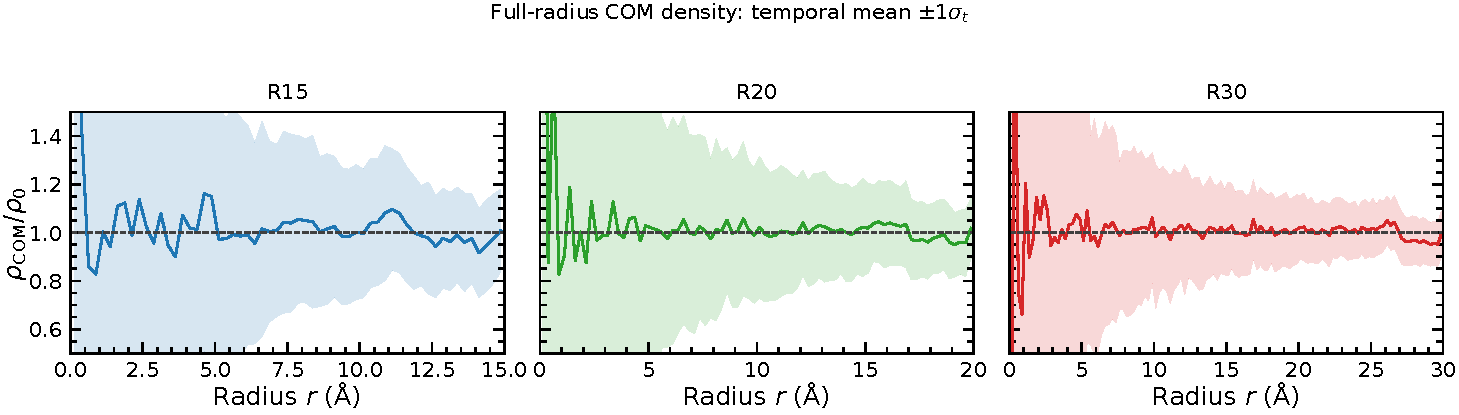
\includegraphics[width=\textwidth,height=0.74\textheight,keepaspectratio]{01_full_radius_density_mean_std.pdf}
\caption{Full-radius molecular-COM density.  Solid lines are temporal means
and shaded bands are the first temporal standard deviation across saved
frames.}
\label{fig:s01-density}
\end{figure}
\clearpage

\begin{figure}[p]
\centering
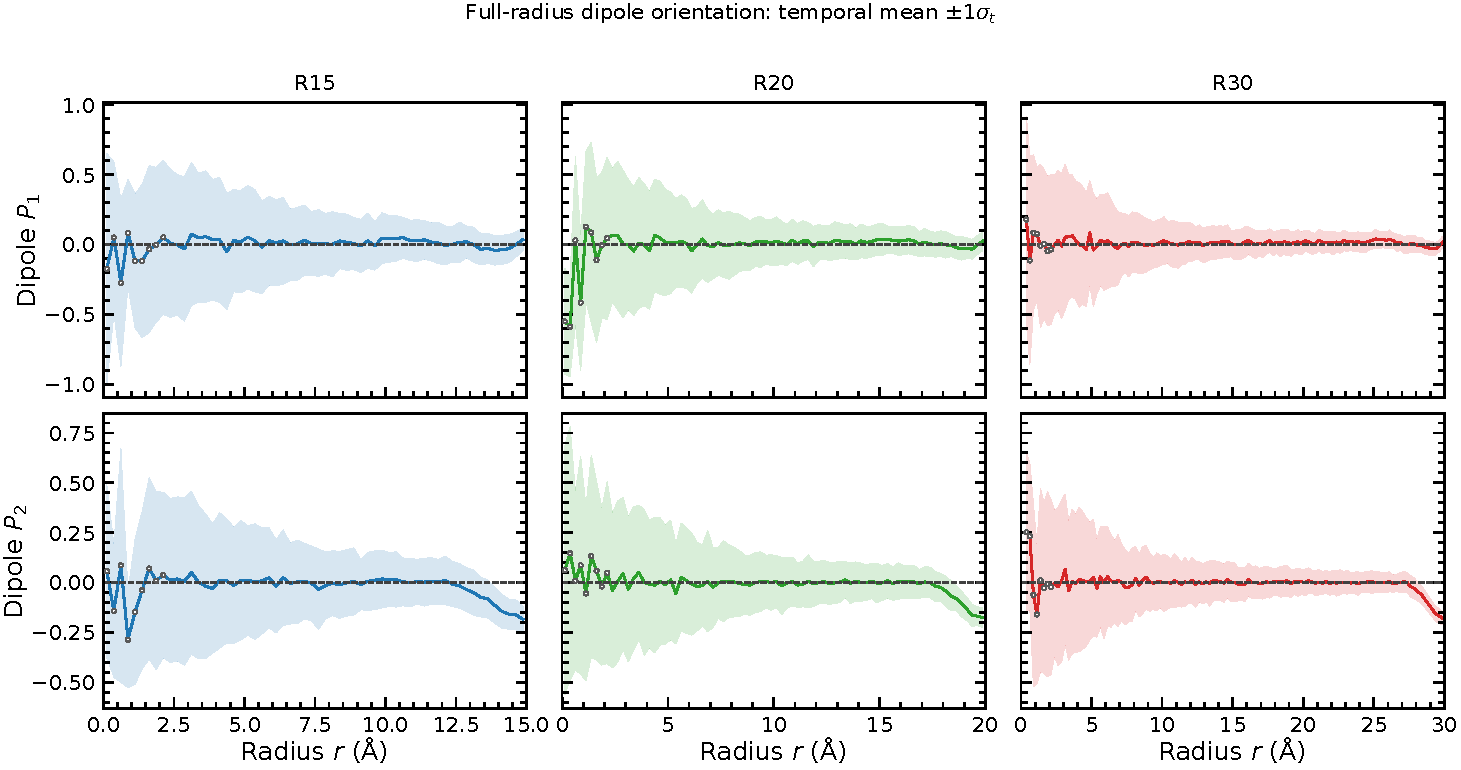
\includegraphics[width=\textwidth,height=0.74\textheight,keepaspectratio]{02_full_radius_orientation_mean_std.pdf}
\caption{Full-radius dipole \(P_1\) and \(P_2\) orientational profiles.  Shaded
bands denote the first temporal standard deviation.}
\label{fig:s02-orientation}
\end{figure}
\clearpage

\begin{figure}[p]
\centering
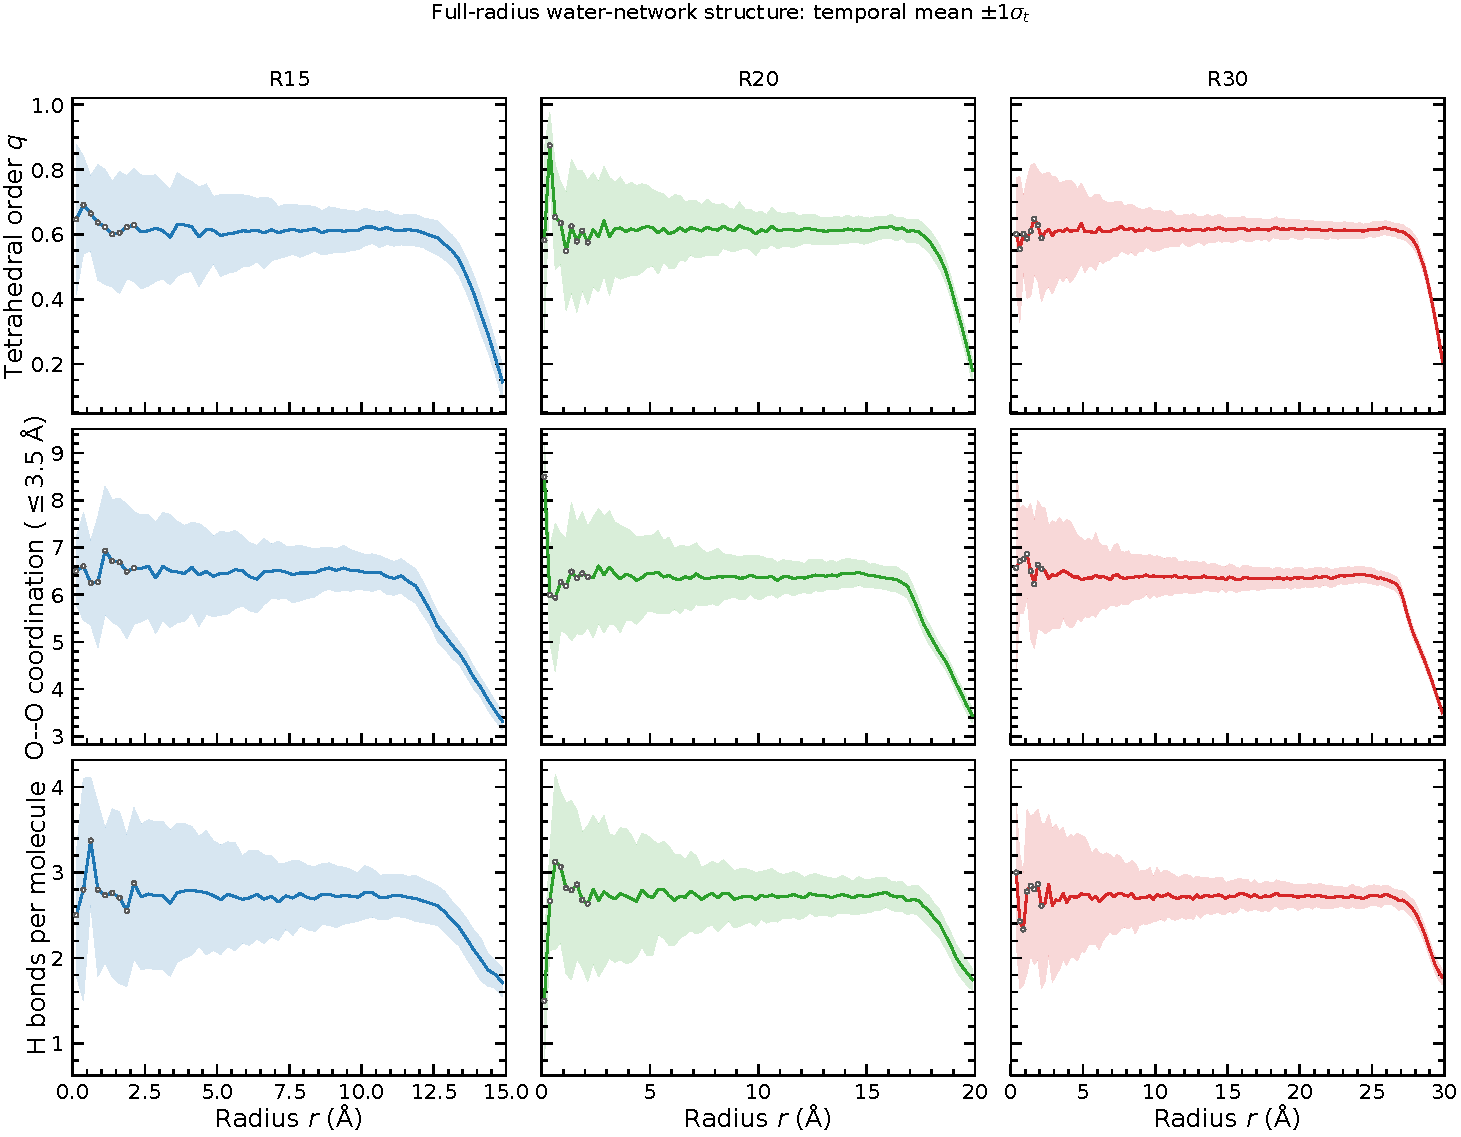
\includegraphics[width=\textwidth,height=0.74\textheight,keepaspectratio]{03_full_radius_network_mean_std.pdf}
\caption{Full-radius tetrahedrality, direct O--O coordination, and hydrogen
bonding profiles.}
\label{fig:s03-network}
\end{figure}
\clearpage

\begin{figure}[p]
\centering
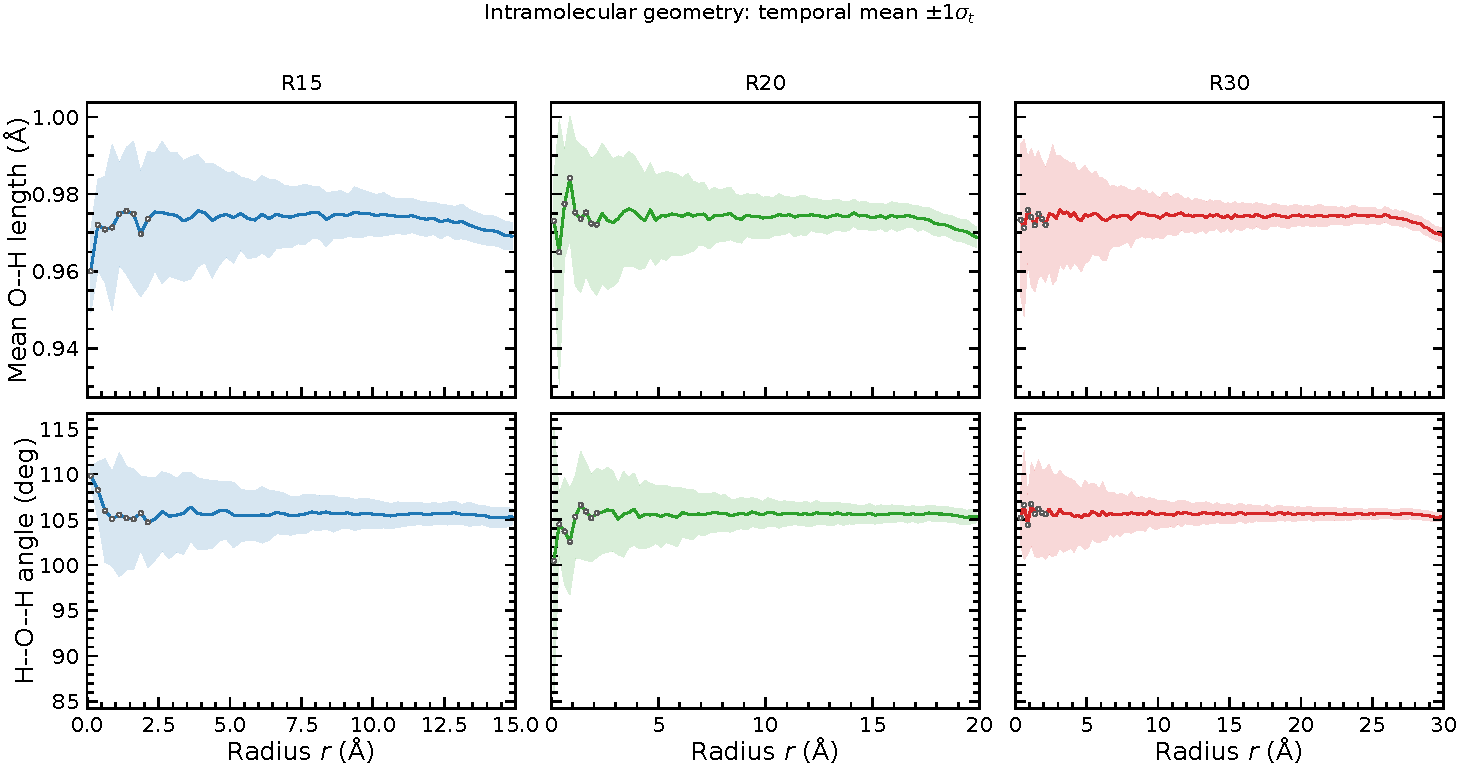
\includegraphics[width=\textwidth,height=0.74\textheight,keepaspectratio]{04_full_radius_intramolecular_geometry_mean_std.pdf}
\caption{Full-radius mean O--H bond length and H--O--H angle profiles.}
\label{fig:s04-intramolecular}
\end{figure}
\clearpage

\begin{figure}[p]
\centering
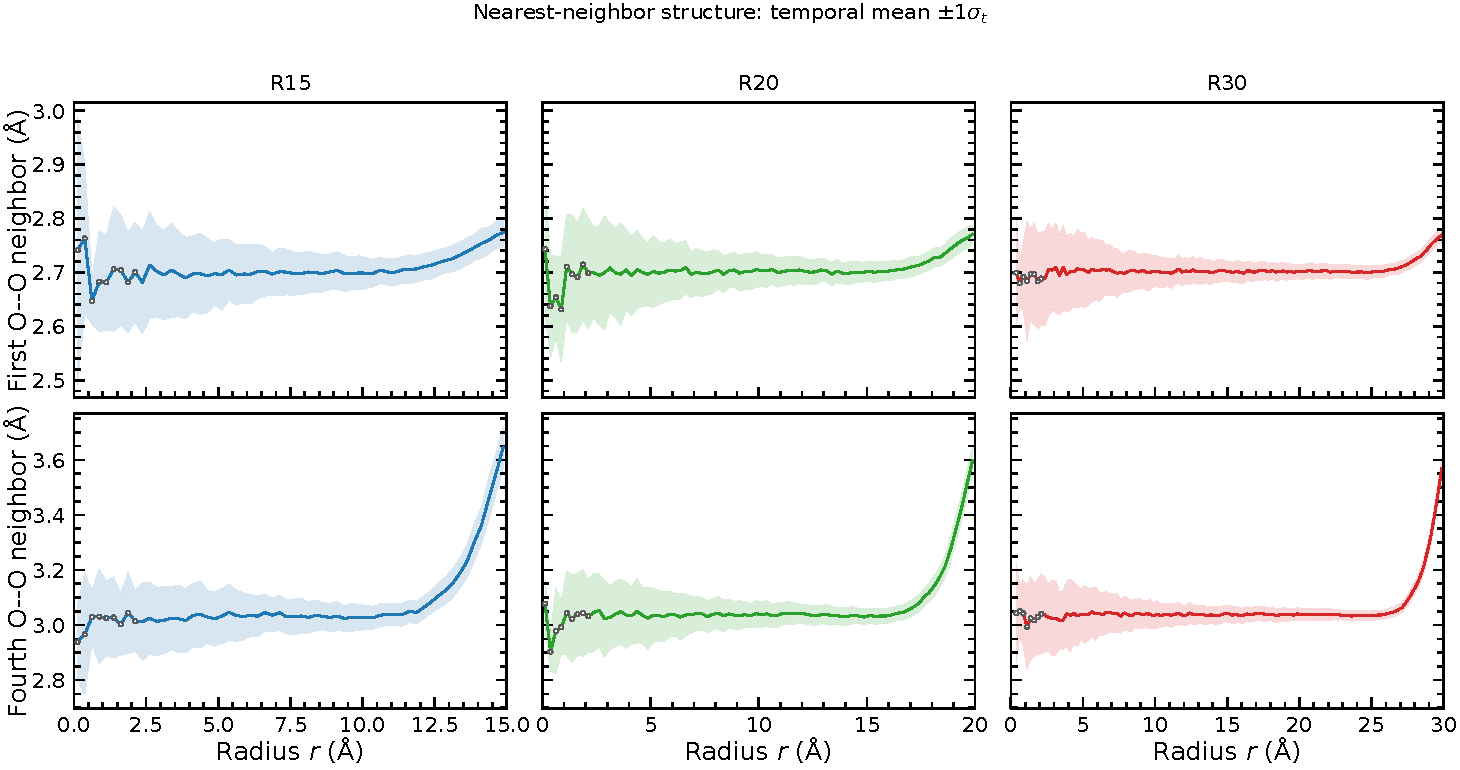
\includegraphics[width=\textwidth,height=0.74\textheight,keepaspectratio]{05_full_radius_nearest_neighbors_mean_std.pdf}
\caption{Full-radius first- and fourth-nearest O--O neighbor-distance
profiles.}
\label{fig:s05-neighbors}
\end{figure}
\clearpage

\begin{figure}[p]
\centering
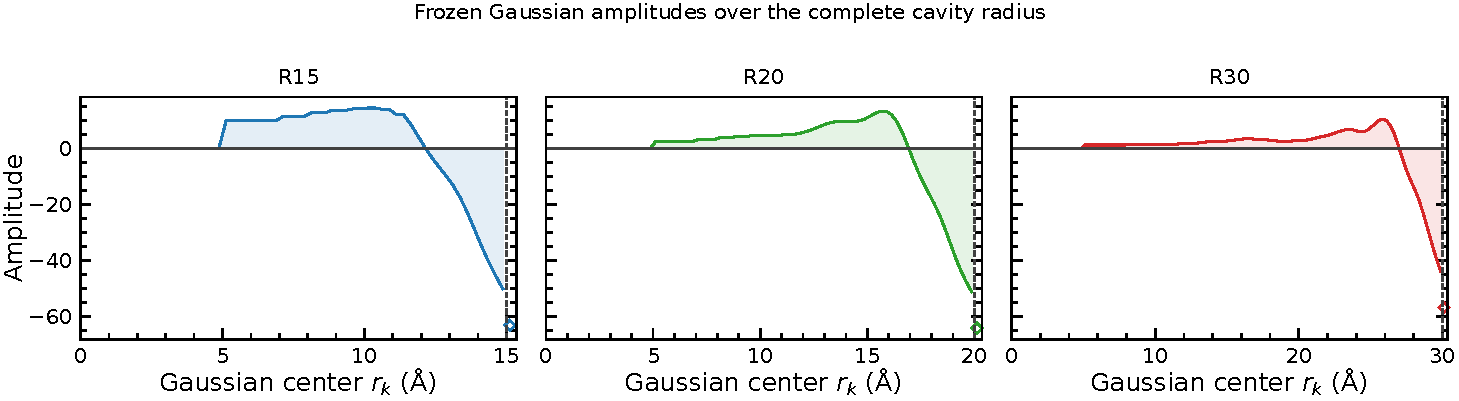
\includegraphics[width=\textwidth,height=0.74\textheight,keepaspectratio]{06_full_radius_gaussian_amplitudes.pdf}
\caption{Frozen physical Gaussian coefficients over the complete absolute
radius.  The open diamond denotes the additional control layer.}
\label{fig:s06-amplitudes}
\end{figure}
\clearpage

\begin{figure}[p]
\centering
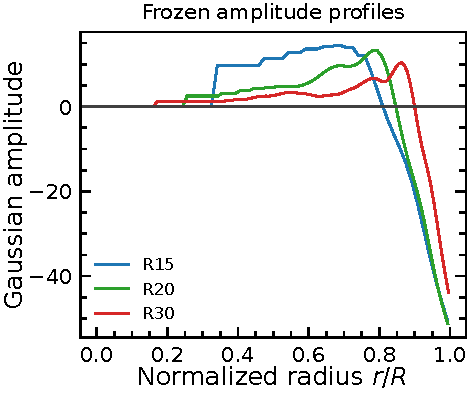
\includegraphics[width=\textwidth,height=0.74\textheight,keepaspectratio]{07_normalized_radius_gaussian_amplitudes.pdf}
\caption{Frozen physical Gaussian coefficients aligned by normalized radius
\(r/R\).}
\label{fig:s07-amplitudes-normalized}
\end{figure}
\clearpage

\begin{figure}[p]
\centering
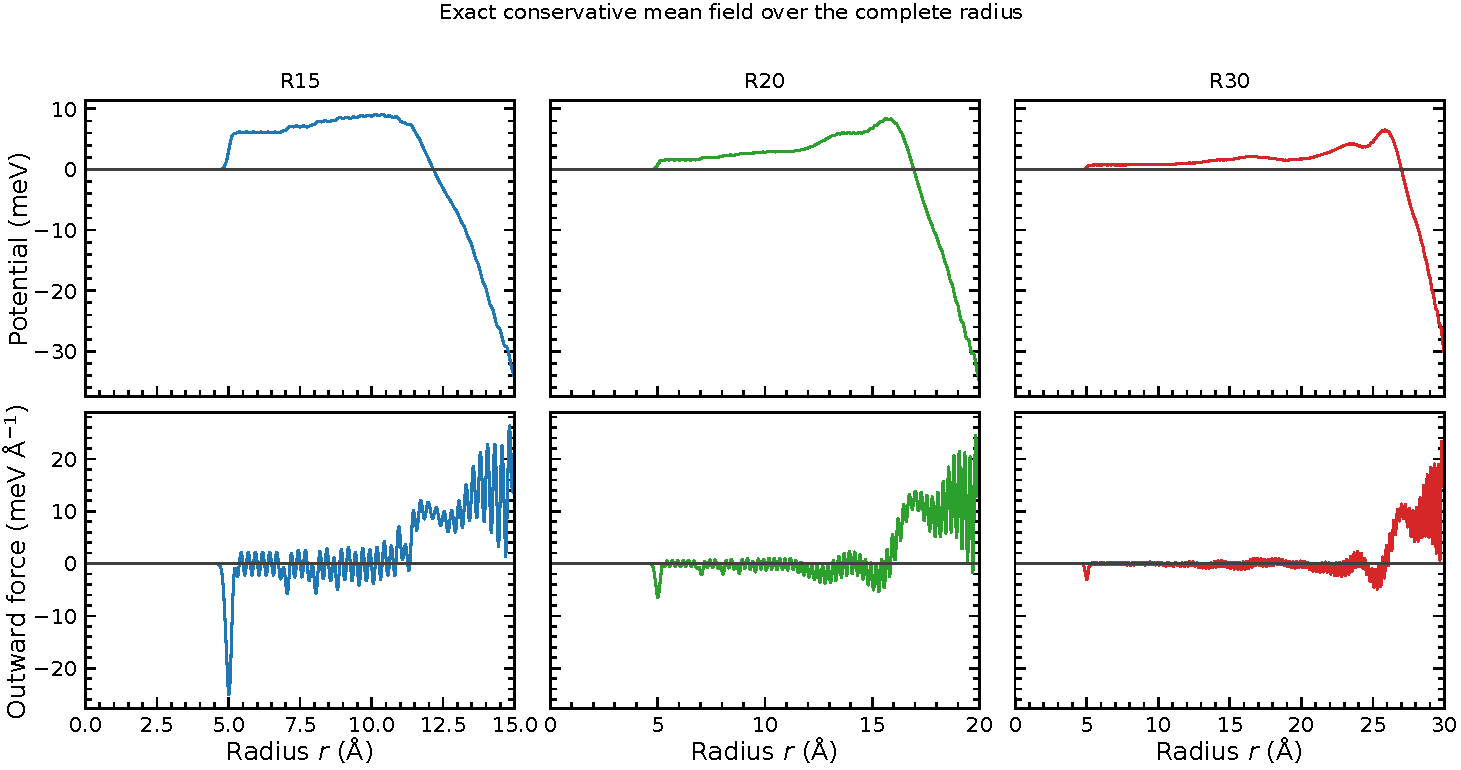
\includegraphics[width=\textwidth,height=0.74\textheight,keepaspectratio]{08_full_radius_potential_and_force.pdf}
\caption{Exact Gaussian-sum potential and its analytic conservative radial
force over the complete interval \(0\leq r\leq R\).}
\label{fig:s08-potential-full}
\end{figure}
\clearpage

\begin{figure}[p]
\centering
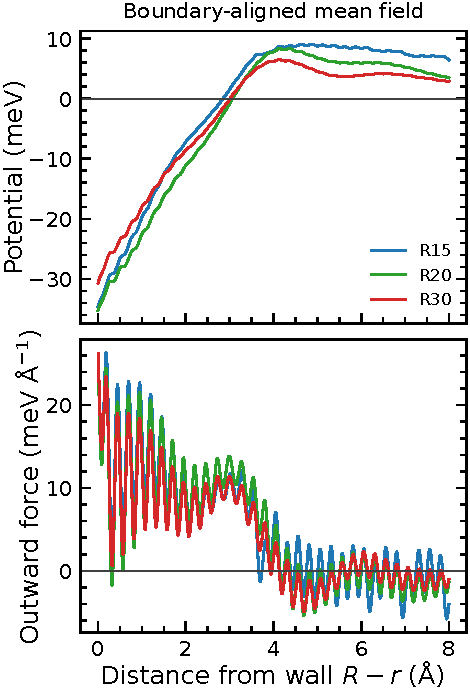
\includegraphics[width=\textwidth,height=0.74\textheight,keepaspectratio]{09_wall_aligned_potential_and_force.pdf}
\caption{Mean-field potential and force aligned by distance from the cavity
wall.}
\label{fig:s09-potential-wall}
\end{figure}
\clearpage

\begin{figure}[p]
\centering
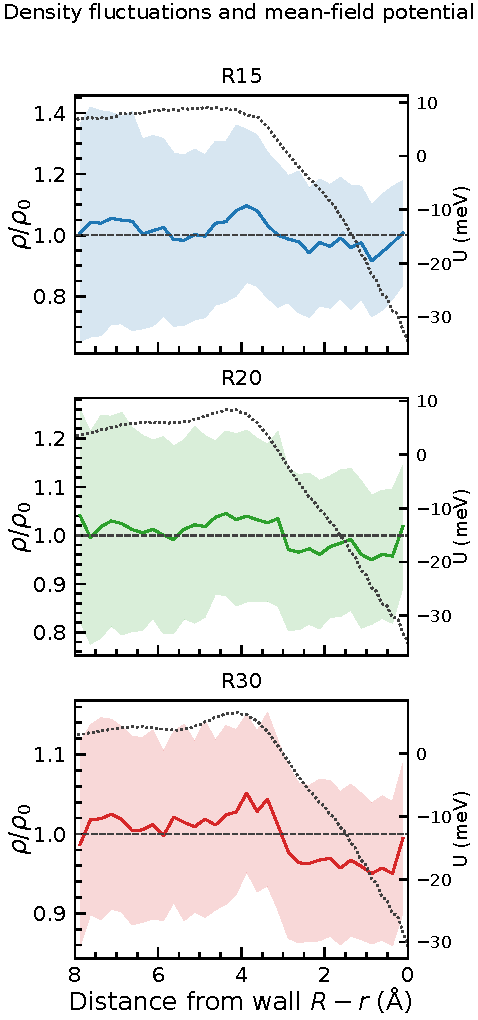
\includegraphics[width=\textwidth,height=0.74\textheight,keepaspectratio]{10_density_fluctuation_potential_overlay.pdf}
\caption{Boundary density mean and first temporal standard deviation overlaid
with the exact mean-field potential (dotted curve, right axis).}
\label{fig:s10-density-potential}
\end{figure}
\clearpage

\begin{figure}[p]
\centering
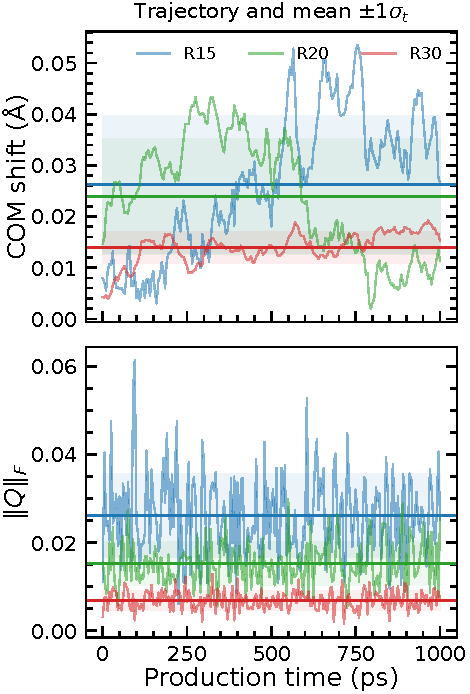
\includegraphics[width=\textwidth,height=0.74\textheight,keepaspectratio]{11_global_temporal_fluctuations.pdf}
\caption{Global molecular-COM displacement and angular-anisotropy time traces,
with temporal mean and first standard deviation.}
\label{fig:s11-global}
\end{figure}
\clearpage

\begin{figure}[p]
\centering
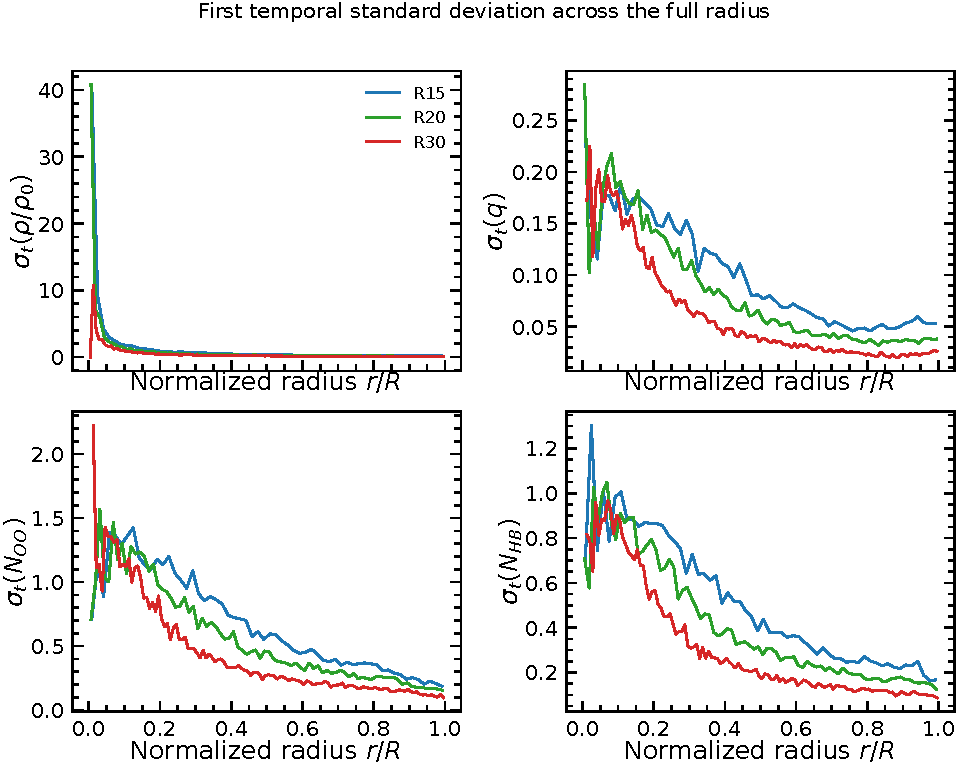
\includegraphics[width=\textwidth,height=0.74\textheight,keepaspectratio]{12_full_radius_temporal_standard_deviation.pdf}
\caption{First temporal standard deviation of density and network observables
over the complete normalized radius.}
\label{fig:s12-temporal-sd}
\end{figure}
\clearpage

\begin{figure}[p]
\centering
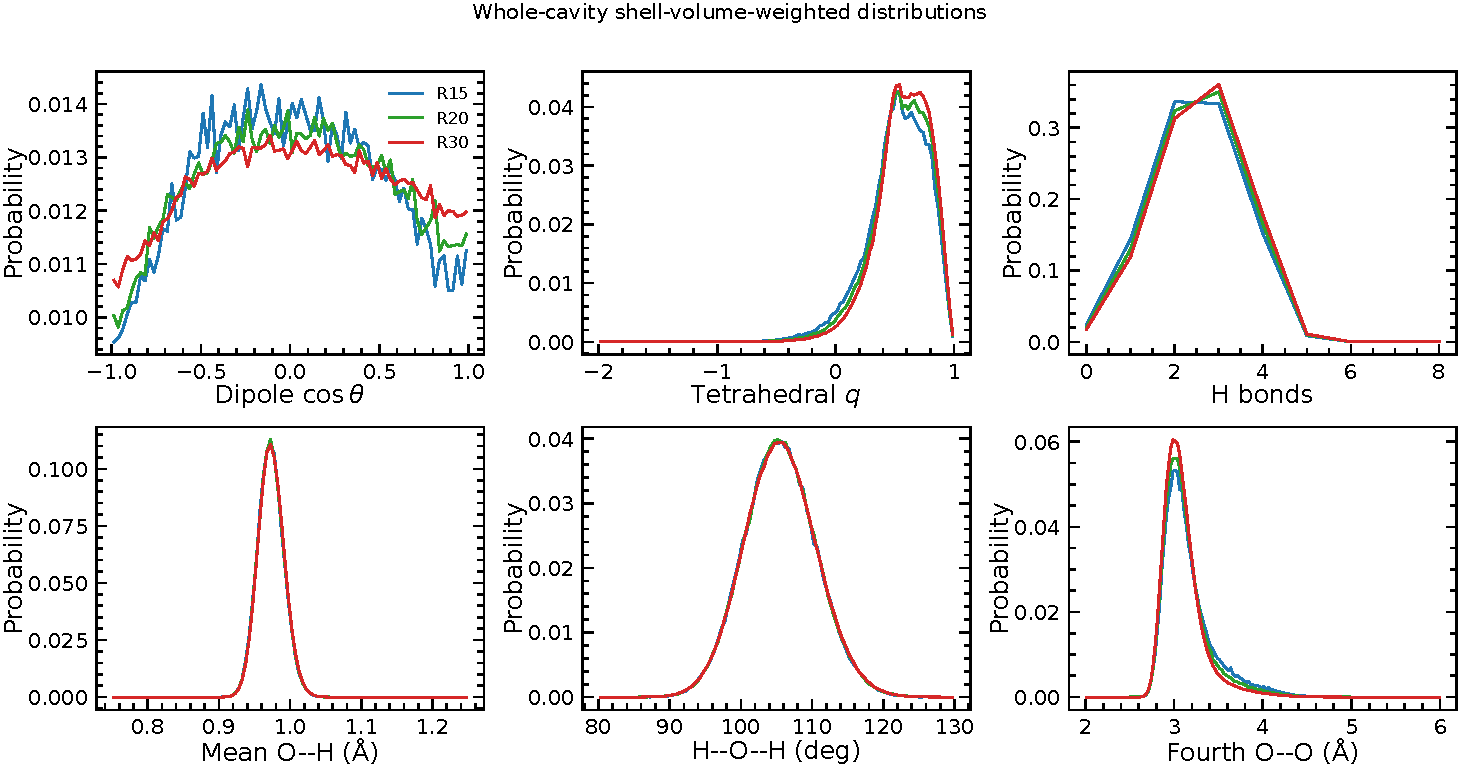
\includegraphics[width=\textwidth,height=0.74\textheight,keepaspectratio]{13_volume_weighted_distributions.pdf}
\caption{Whole-cavity shell-volume-weighted distributions of molecular
coordinates and structural observables.}
\label{fig:s13-distributions}
\end{figure}
\clearpage

\begin{figure}[p]
\centering
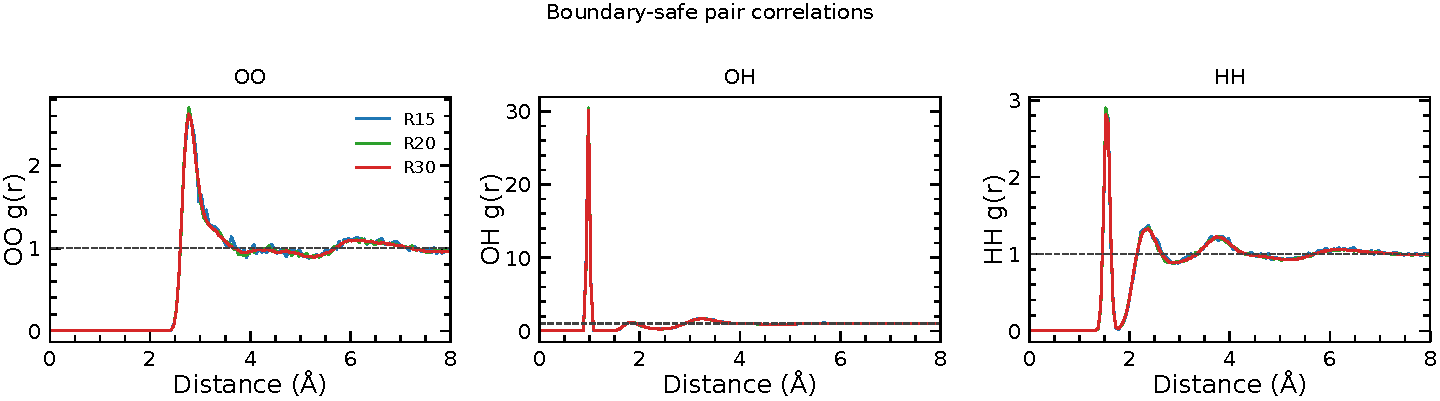
\includegraphics[width=\textwidth,height=0.74\textheight,keepaspectratio]{14_boundary_safe_pair_correlations.pdf}
\caption{Boundary-safe total O--O, O--H, and H--H radial distribution
functions.  Intramolecular contributions are retained for O--H and H--H.}
\label{fig:s14-rdf-total}
\end{figure}
\clearpage

\begin{figure}[p]
\centering
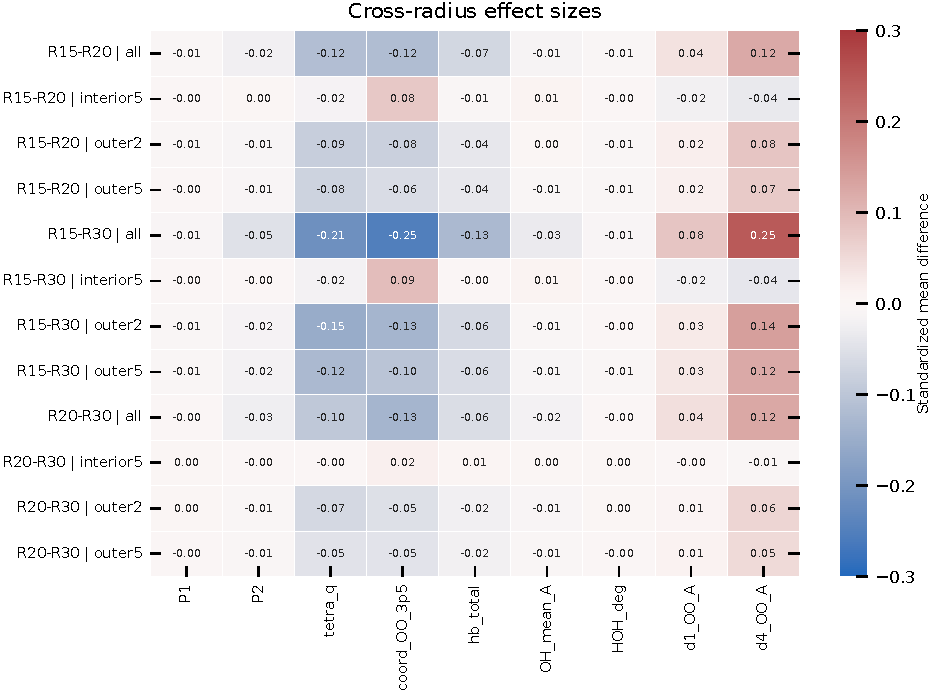
\includegraphics[width=\textwidth,height=0.74\textheight,keepaspectratio]{15_equivalence_effect_size_matrix.pdf}
\caption{Shell-volume-weighted standardized mean differences between cavity
radii, resolved by region and observable.}
\label{fig:s15-equivalence-smd}
\end{figure}
\clearpage

\begin{figure}[p]
\centering
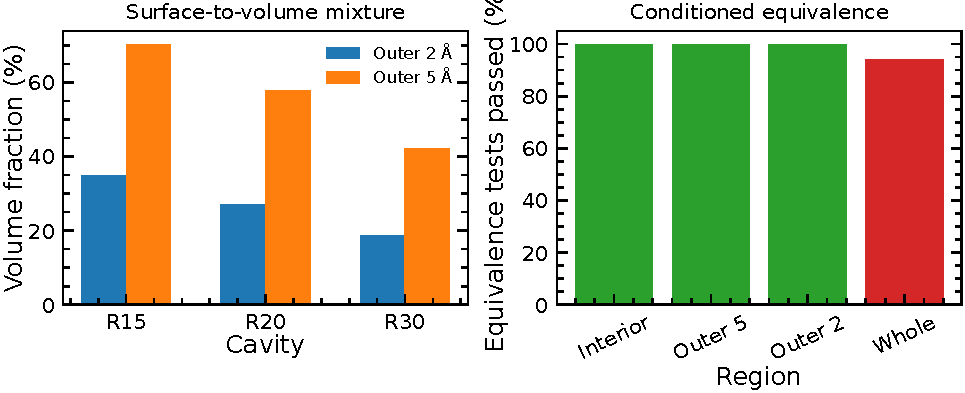
\includegraphics[width=\textwidth,height=0.74\textheight,keepaspectratio]{16_geometric_mixing_and_equivalence.pdf}
\caption{Exact surface-volume fractions and the fraction of practical-
equivalence tests satisfying all four criteria.}
\label{fig:s16-equivalence-geometry}
\end{figure}
\clearpage

\begin{figure}[p]
\centering
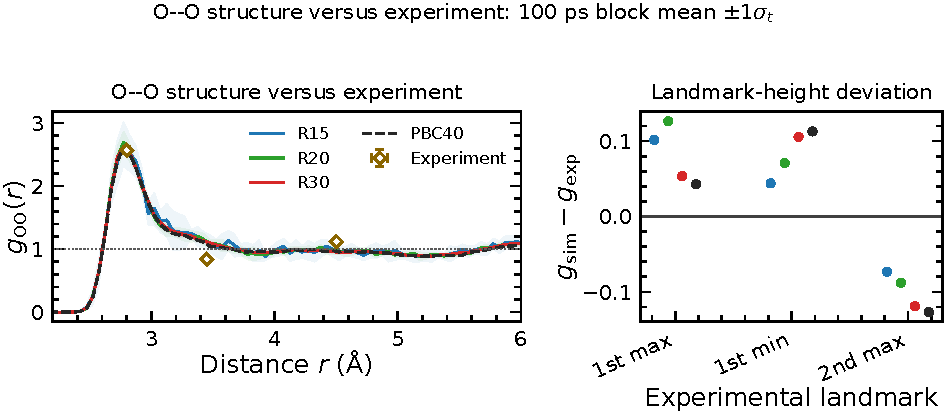
\includegraphics[width=\textwidth,height=0.74\textheight,keepaspectratio]{17_gOO_experimental_benchmark.pdf}
\caption{Intermolecular O--O structure compared with experimental feature
landmarks.  Same-molecule pairs are excluded where applicable; shading is the
first temporal standard deviation across 100 ps RDF blocks.}
\label{fig:s17-goo-exp}
\end{figure}
\clearpage

\begin{figure}[p]
\centering
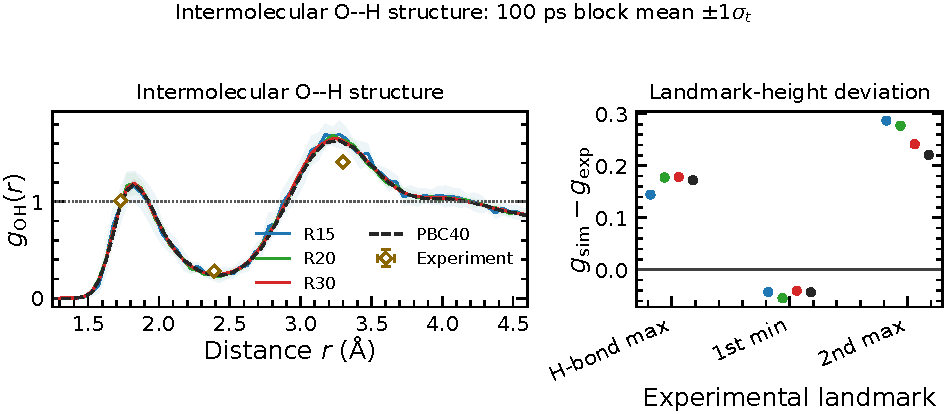
\includegraphics[width=\textwidth,height=0.74\textheight,keepaspectratio]{18_intermolecular_gOH.pdf}
\caption{Intermolecular O--H structure compared with published feature
landmarks.  Same-molecule pairs are excluded; shading is the first temporal
standard deviation across 100 ps RDF blocks.}
\label{fig:s18-goh-exp}
\end{figure}
\clearpage

\begin{figure}[p]
\centering
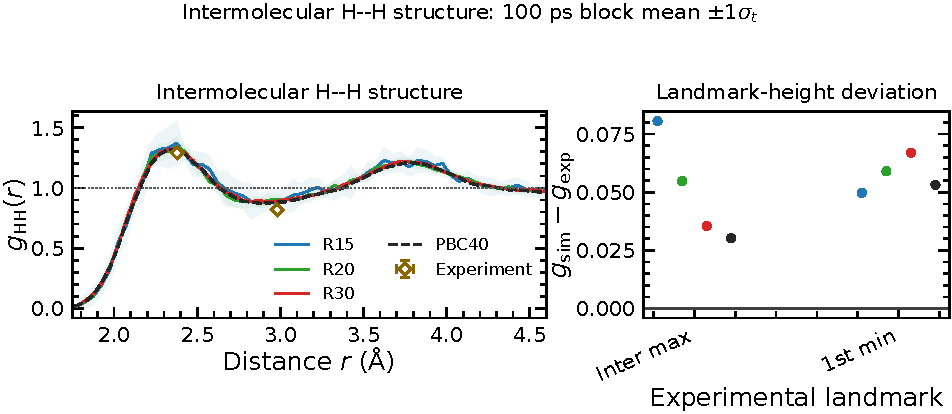
\includegraphics[width=\textwidth,height=0.74\textheight,keepaspectratio]{19_intermolecular_gHH.pdf}
\caption{Intermolecular H--H structure compared with published feature
landmarks.  Same-molecule pairs are excluded; shading is the first temporal
standard deviation across 100 ps RDF blocks.}
\label{fig:s19-ghh-exp}
\end{figure}
\clearpage

\begin{figure}[p]
\centering
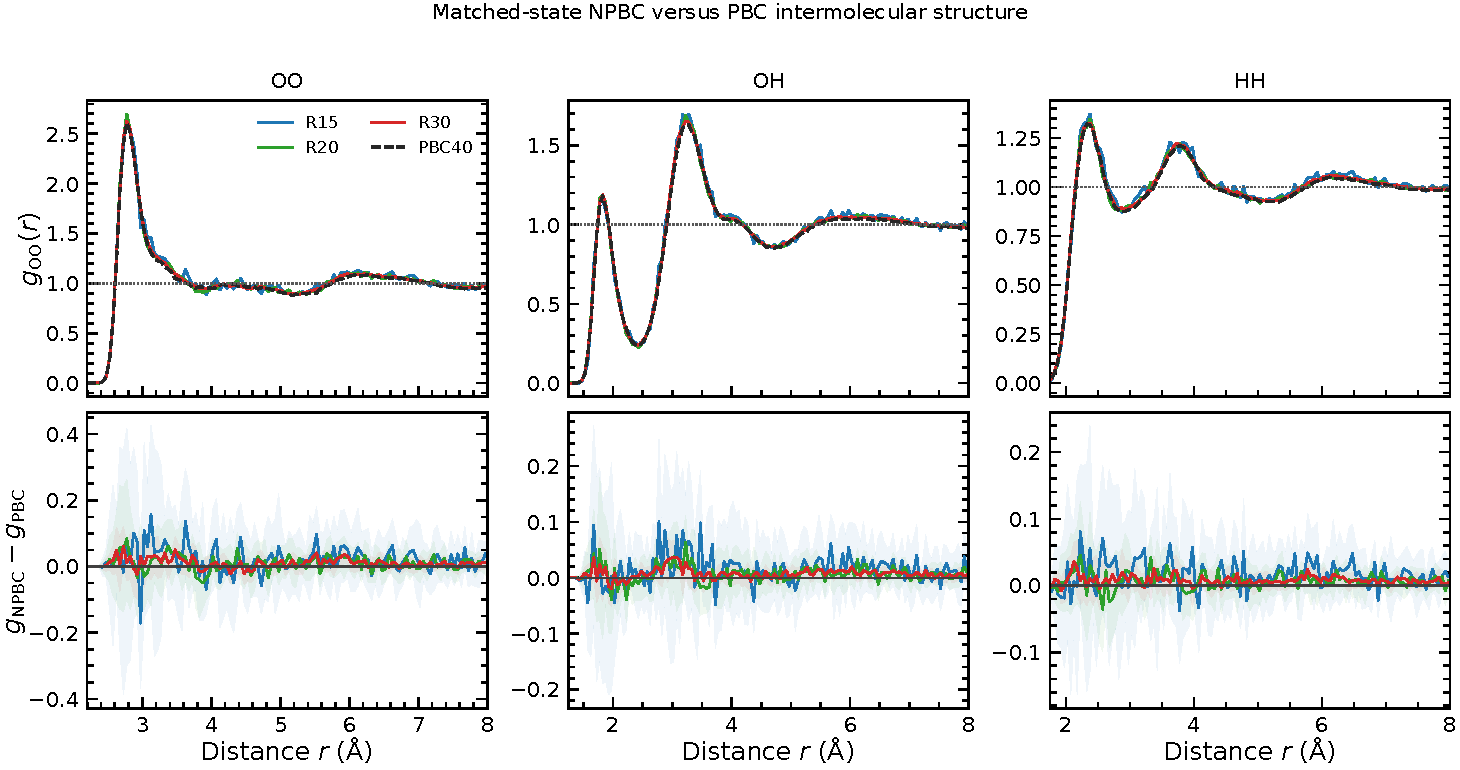
\includegraphics[width=\textwidth,height=0.74\textheight,keepaspectratio]{20_npbc_vs_pbc_rdf.pdf}
\caption{Direct comparison of R15, R20, and R30 with the matched 40
\(\angstrom\) periodic MACE--OFF23 reference.  Residual shading is the
quadrature-combined first temporal standard deviation of the NPBC and PBC
100 ps block RDFs.}
\label{fig:s20-npbc-pbc}
\end{figure}
\clearpage

\begin{figure}[p]
\centering
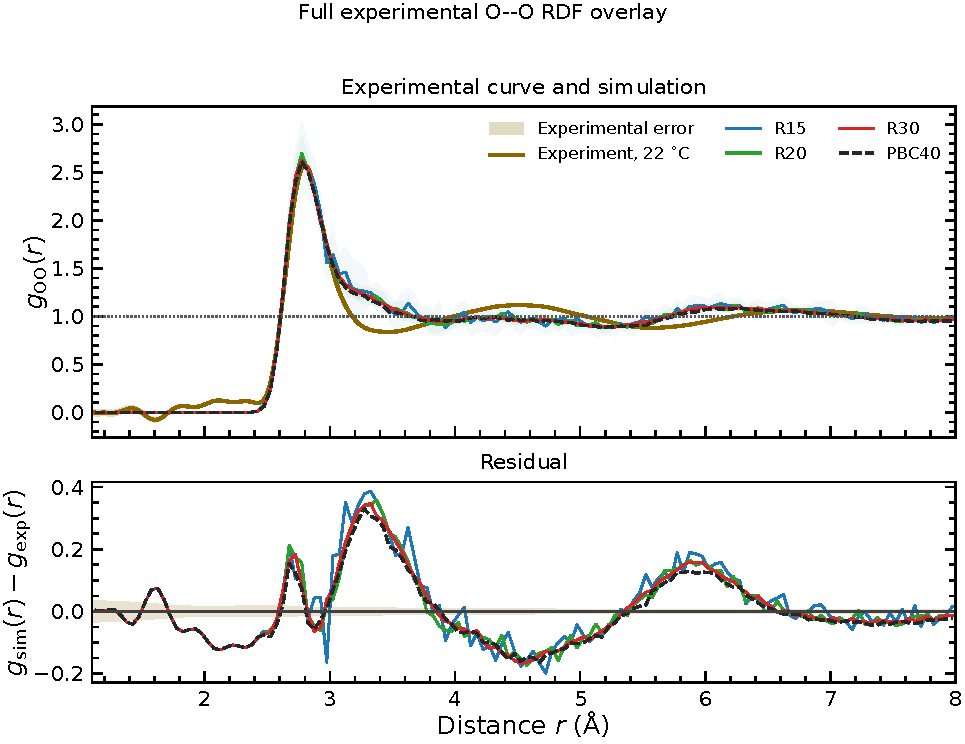
\includegraphics[width=\textwidth,height=0.74\textheight,keepaspectratio]{21_full_experimental_gOO_overlay.pdf}
\caption{Full common-range O--O RDF overlay for R15, R20, R30, and PBC40 with
the Skinner \emph{et al.} experimental curve and its pointwise estimated
error.  Simulation bands are first temporal standard deviations across
100 ps blocks; the lower panel is simulation minus experiment.}
\label{fig:s21-goo-full-exp}
\end{figure}
\clearpage

\begin{figure}[p]
\centering
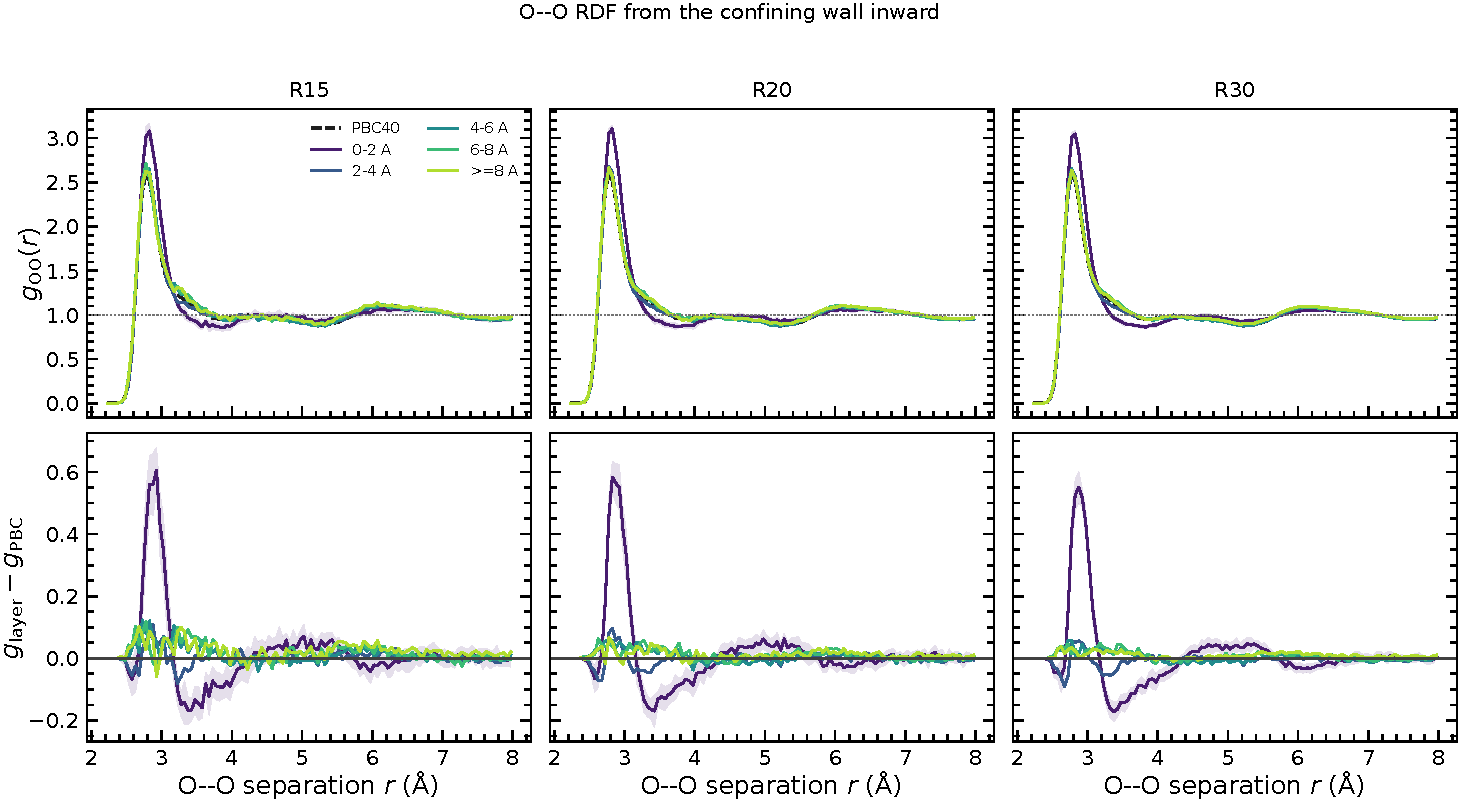
\includegraphics[width=\textwidth,height=0.74\textheight,keepaspectratio]{22_radial_layer_gOO_vs_pbc.pdf}
\caption{O--O RDF conditioned on reference-water COM wall distance.  NPBC
curves use the exact spherical accessible-shell-volume correction and
distinct-particle finite-\(N\) normalization.  Shading is the first temporal
standard deviation across equal 100 ps blocks for PBC and the outer 0--2
\(\angstrom\) layer.}
\label{fig:s22-radial-goo}
\end{figure}
\clearpage

\begin{figure}[p]
\centering
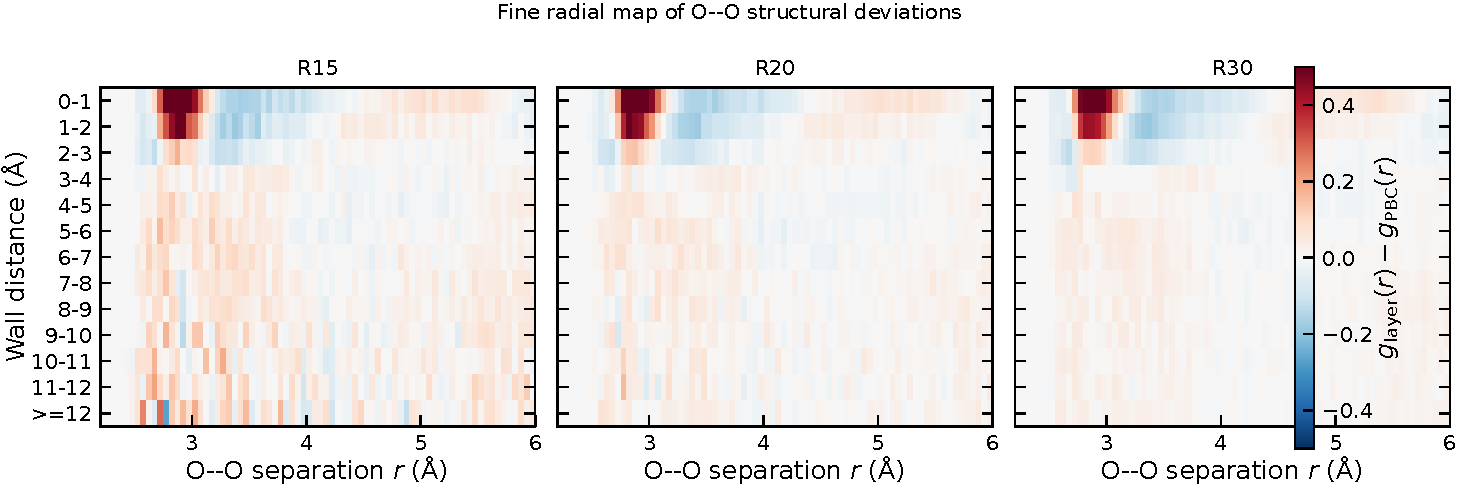
\includegraphics[width=\textwidth,height=0.74\textheight,keepaspectratio]{23_radial_layer_gOO_delta_heatmap.pdf}
\caption{Fine 1 \(\angstrom\) wall-layer heat map of the edge-corrected
\(g_{\OO,L}(r)-g_{\OO,\PBC}(r)\).  Rows run from the outer wall inward.}
\label{fig:s23-radial-goo-heatmap}
\end{figure}
\clearpage

\begin{figure}[p]
\centering
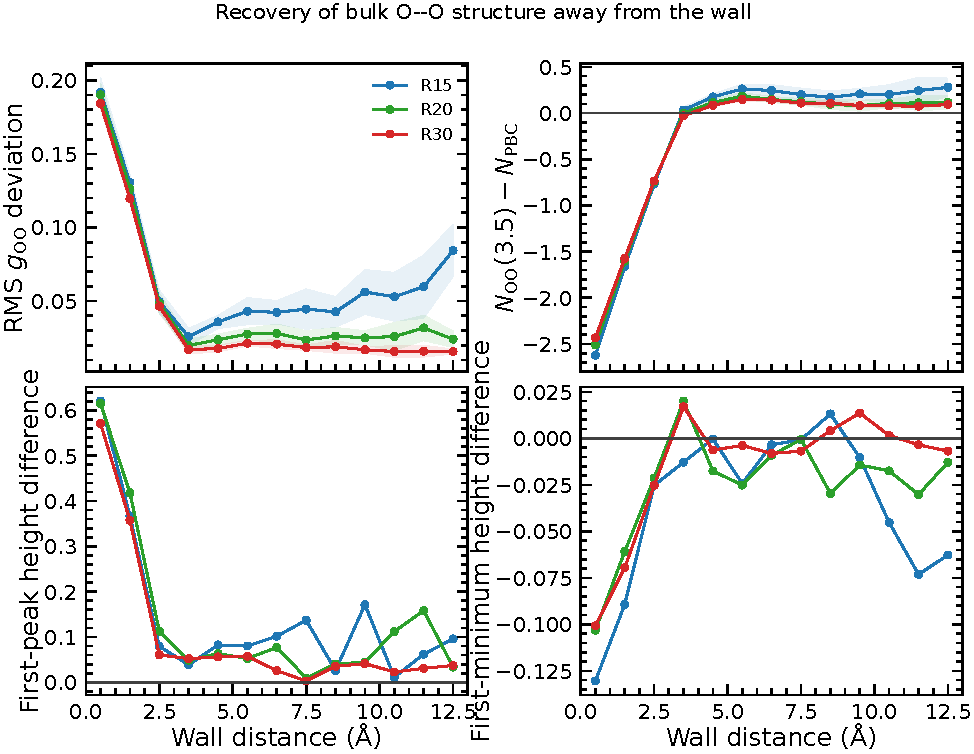
\includegraphics[width=\textwidth,height=0.74\textheight,keepaspectratio]{24_radial_layer_gOO_metrics.pdf}
\caption{Fine-layer RDF deviation metrics versus distance from the wall.
Shading on RDF RMSE and direct coordination is the first temporal standard
deviation across equal 100 ps blocks.}
\label{fig:s24-radial-goo-metrics}
\end{figure}
\clearpage

\begin{figure}[p]
\centering
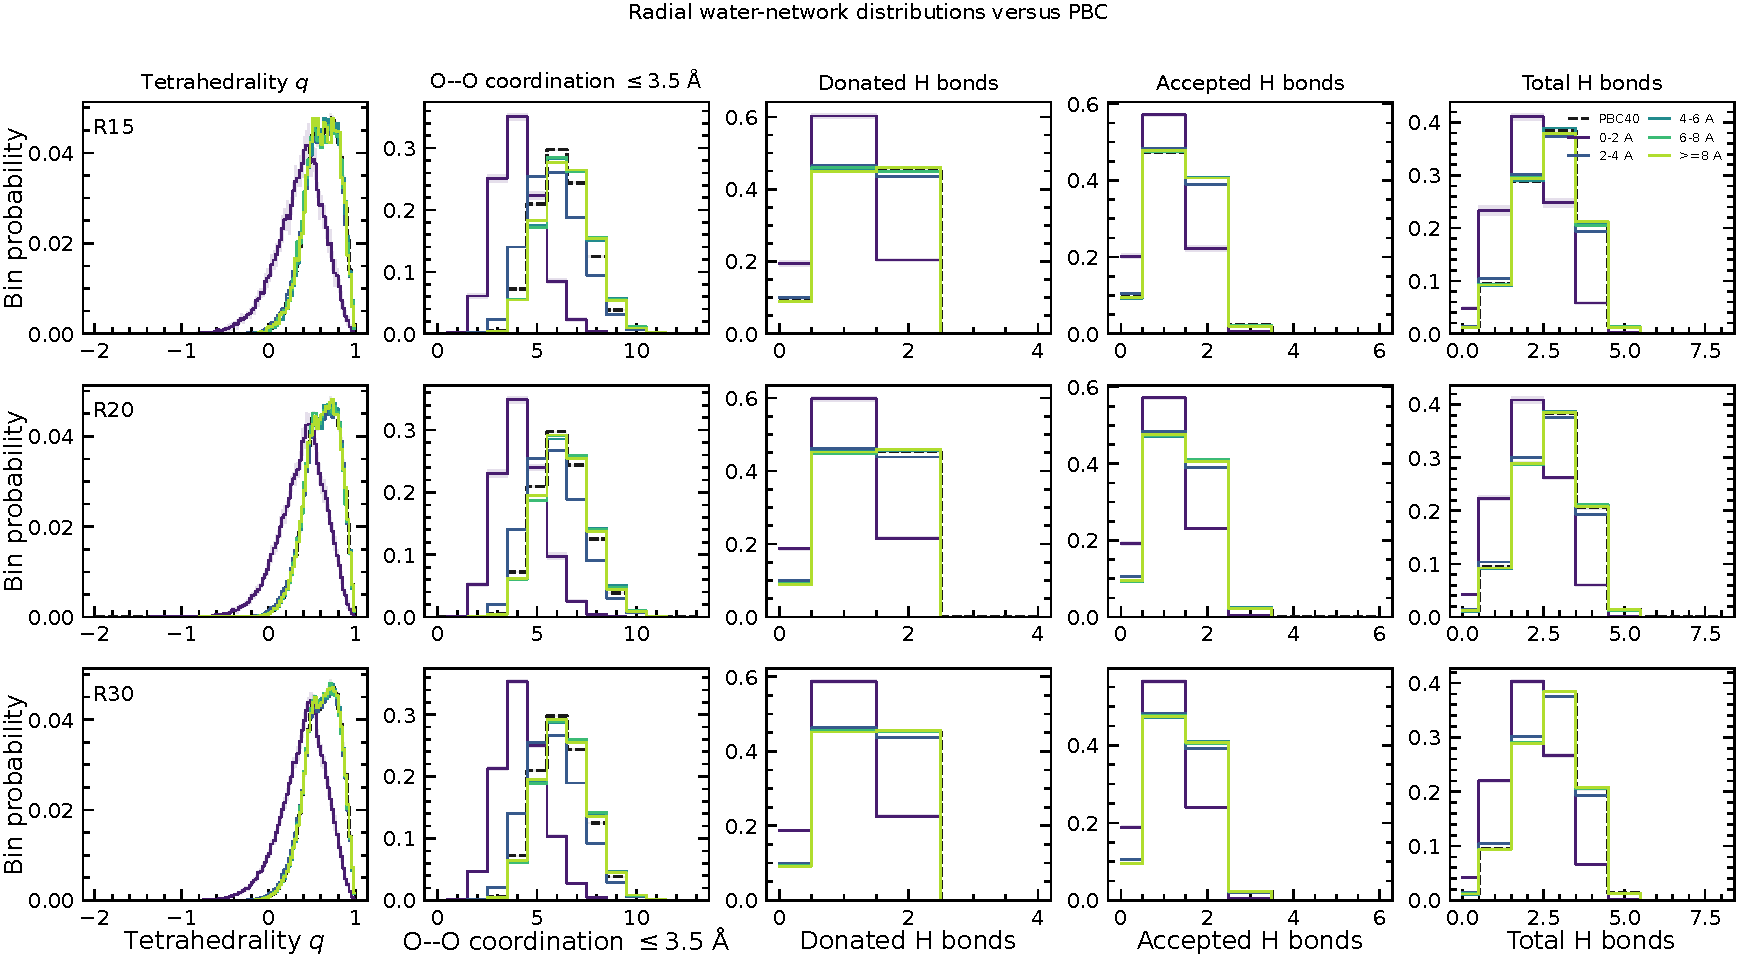
\includegraphics[width=\textwidth,height=0.74\textheight,keepaspectratio]{25_radial_layer_network_distributions_vs_pbc.pdf}
\caption{Radial water-network distributions compared with PBC.  Histograms
are molecule-weighted in 2 \(\angstrom\) wall-distance layers.  Shading is the
first temporal standard deviation across equal 100 ps blocks for PBC and the
outer 0--2 \(\angstrom\) layer.}
\label{fig:s25-network-hists}
\end{figure}
\clearpage

\begin{figure}[p]
\centering
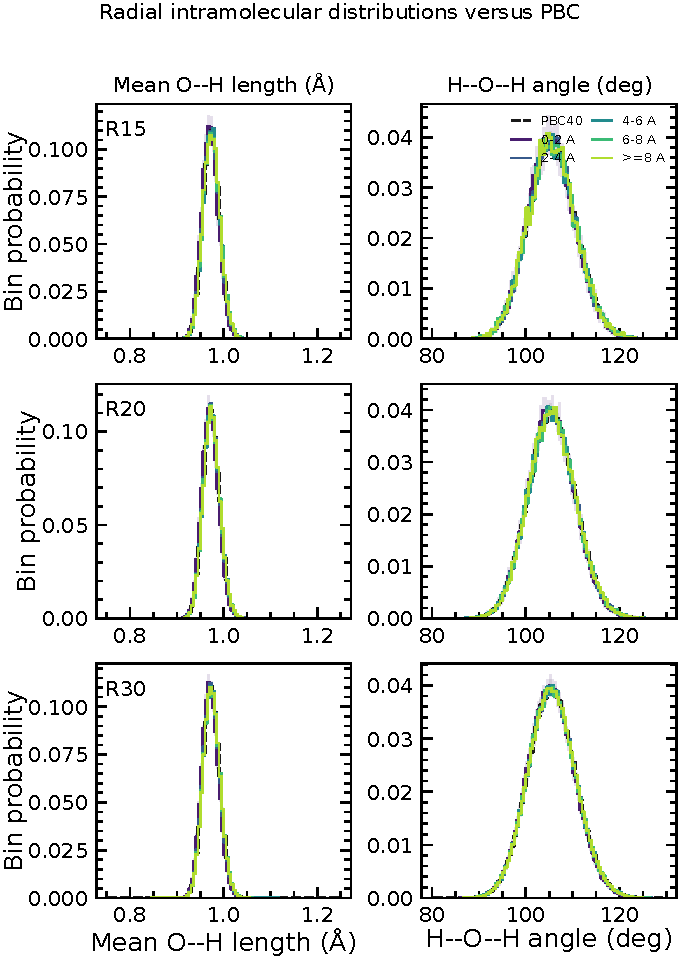
\includegraphics[width=\textwidth,height=0.74\textheight,keepaspectratio]{26_radial_layer_intramolecular_distributions_vs_pbc.pdf}
\caption{Radial intramolecular O--H length and H--O--H angle distributions
compared with PBC.  Histograms are molecule-weighted in 2 \(\angstrom\)
wall-distance layers; shading follows the convention in
\cref{fig:s25-network-hists}.}
\label{fig:s26-intra-hists}
\end{figure}
\clearpage

\begin{figure}[p]
\centering
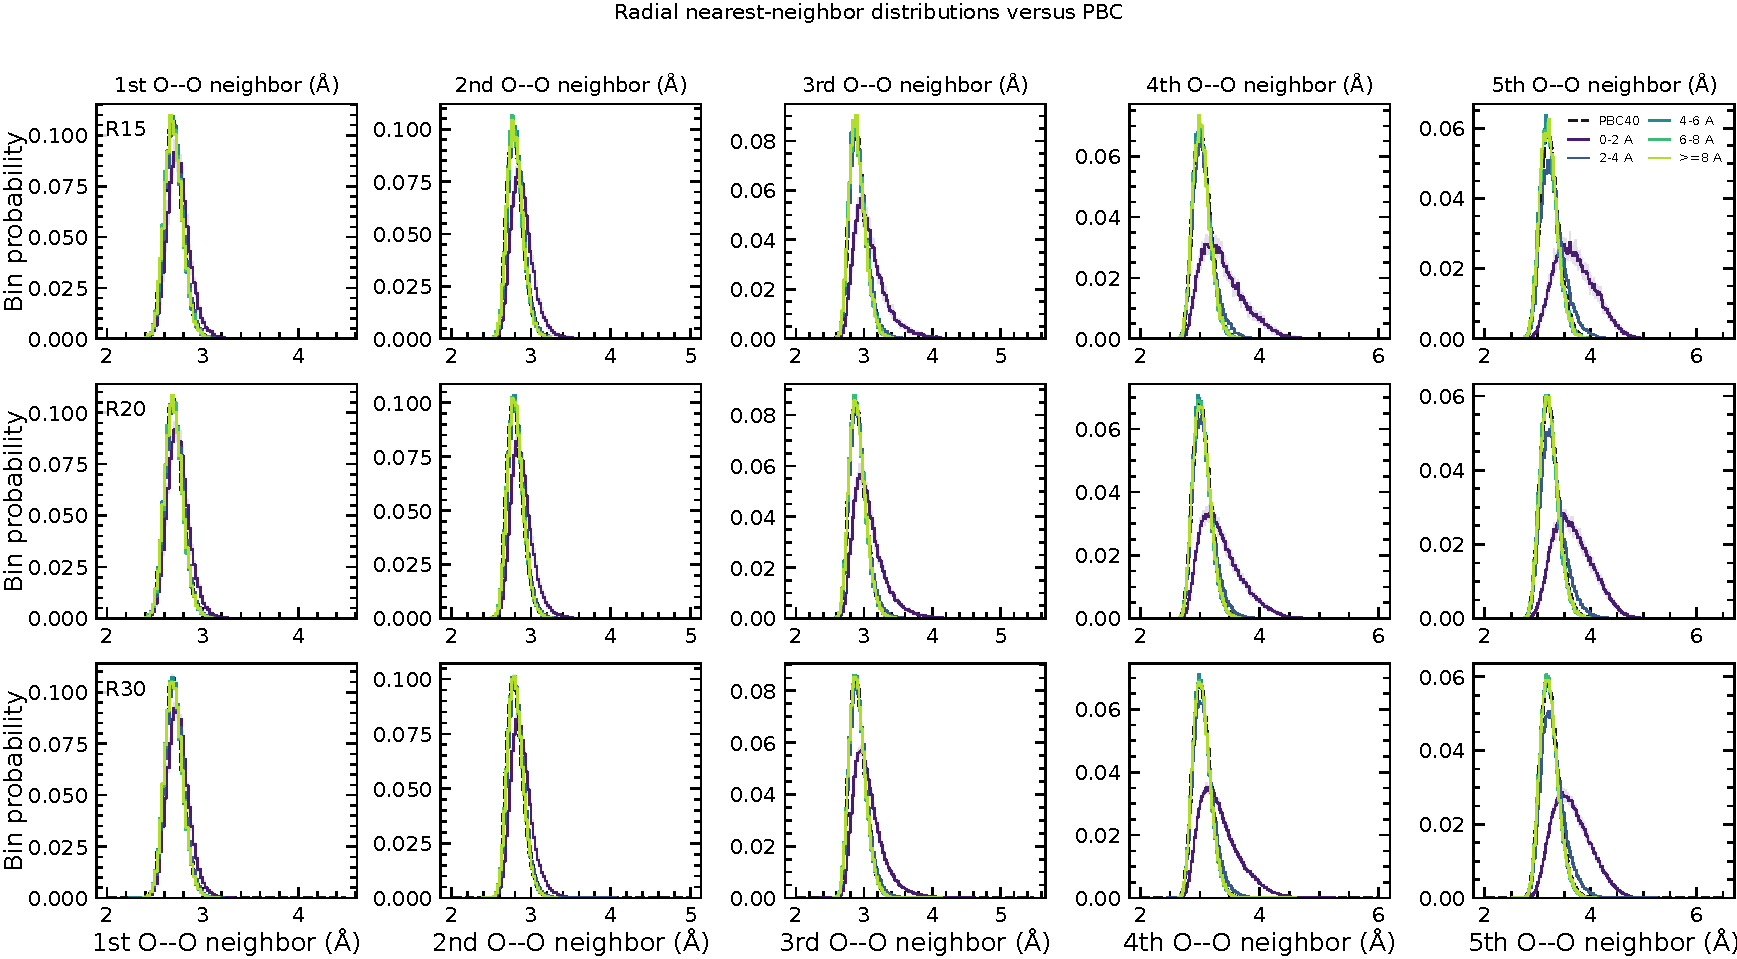
\includegraphics[width=\textwidth,height=0.74\textheight,keepaspectratio]{27_radial_layer_neighbor_distributions_vs_pbc.pdf}
\caption{First-through-fifth O--O-neighbor distributions by radial layer and
PBC.  Histograms are molecule-weighted in 2 \(\angstrom\) wall-distance
layers; shading follows the convention in \cref{fig:s25-network-hists}.}
\label{fig:s27-neighbor-hists}
\end{figure}
\clearpage

\begin{figure}[p]
\centering
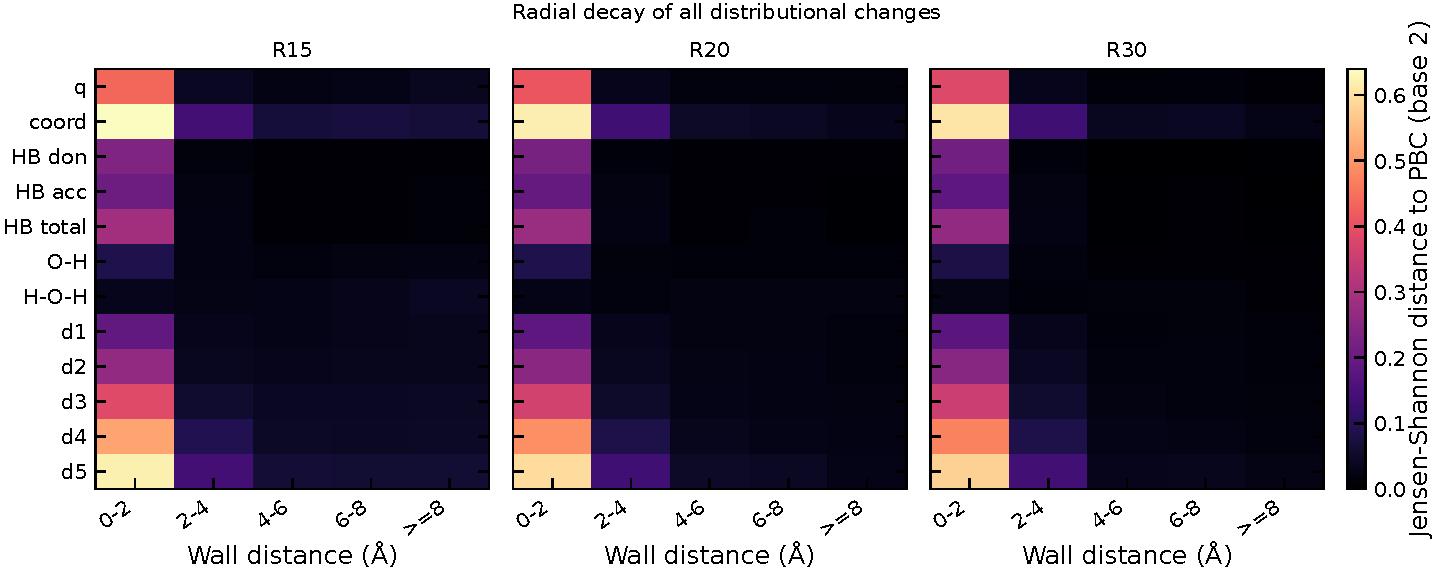
\includegraphics[width=\textwidth,height=0.74\textheight,keepaspectratio]{28_radial_layer_distribution_js_heatmap.pdf}
\caption{Base-2 Jensen--Shannon distance between each shell-conditioned
intrinsic-property histogram and the matched PBC40 histogram.  Zero denotes
identical binned distributions.}
\label{fig:s28-js}
\end{figure}
\clearpage

\end{document}
